\documentclass{tufte-handout}

%\geometry{showframe}% for debugging purposes -- displays the margins

\usepackage{amsmath}


% Set up the images/graphics package
\usepackage{graphicx}
\setkeys{Gin}{width=\linewidth,totalheight=\textheight,keepaspectratio}
\graphicspath{{graphics/}}


% The following package makes prettier tables.  We're all about the bling!
\usepackage{booktabs}

% The units package provides nice, non-stacked fractions and better spacing
% for units.
\usepackage{units}

% The fancyvrb package lets us customize the formatting of verbatim
% environments.  We use a slightly smaller font.
\usepackage{fancyvrb}
\fvset{fontsize=\normalsize}

% Small sections of multiple columns
\usepackage{multicol}

% Provides paragraphs of dummy text
\usepackage{lipsum}

% Provides annotated music scores
\usepackage{musicography}

% Fancy header
\usepackage{fancyhdr}

\usepackage{array, boldline, makecell, booktabs}

\newcommand{\bmp}[1]{\begin{minipage}{#1}}
\newcommand{\emp}{\end{minipage}}
\newcommand{\tw}{\textwidth}

% These commands are used to pretty-print LaTeX commands
\newcommand{\doccmd}[1]{\texttt{\textbackslash#1}}% command name -- adds backslash automatically
\newcommand{\docopt}[1]{\ensuremath{\langle}\textrm{\textit{#1}}\ensuremath{\rangle}}% optional command argument
\newcommand{\docarg}[1]{\textrm{\textit{#1}}}% (required) command argument
\newenvironment{docspec}{\begin{quote}\noindent}{\end{quote}}% command specification environment
\newcommand{\docenv}[1]{\textsf{#1}}% environment name
\newcommand{\docpkg}[1]{\texttt{#1}}% package name
\newcommand{\doccls}[1]{\texttt{#1}}% document class name
\newcommand{\docclsopt}[1]{\texttt{#1}}% document class option name


%%% Additions to template by DSL
\usepackage{hyperref} % provides \url{}
% remove separation between list items http://tex.stackexchange.com/a/10689/1783
\usepackage{enumitem}
\setlist{nosep}

%%-- another way
\usepackage{tikzpagenodes}
\newcommand{\mylogo}[1]{%
\tikz[remember picture,overlay] {%
  \node[inner sep=0pt,anchor=east] at ([yshift=+1.0cm, xshift=+7.0cm]current page text area.north east){#1};}
  }

\usepackage{mathrsfs}
\usepackage{tcolorbox}
\tcbuselibrary{theorems}
\usepackage{xcolor}
\usepackage{epsdice}
\usepackage{pgfplots}

\usepackage{graphicx,xspace,color,cancel}
\usepackage{tikz}
\usetikzlibrary{arrows,shapes,backgrounds,through,shadows}
\usetikzlibrary{decorations.pathmorphing}
\usetikzlibrary{calc}

\newcommand{\boxit}[4]
{
\path #2+(-#4,-#4) node(bottomleft){};
\path #3+(#4,#4) node(upperright){};
\draw[rounded corners,black!80] (bottomleft) rectangle (upperright);
%\path (#2-|#3) node(bottomright){};
\path (bottomleft-|upperright) node(bottomright){};
\path (bottomright) node[above left]{#1};
}

\tikzstyle{cont}=[circle, draw,% a shading that is white at the top...
thick,minimum size=6mm,line width=1pt,>=stealth]  % continuous  node
\tikzstyle{dgraph}=[->, line width=1.5pt]

\tikzstyle{contblk}=[circle, draw=black,top color=black,bottom color=black,% a shading that is white at the top...
thick,minimum size=1mm,line width=1pt,>=stealth]  % continuous  node
\tikzstyle{dgraph}=[->, line width=1.5pt]



\newtcbtheorem[number within=]{mydef}{Definition}%
{colback=DarkOrchid!5,colframe=DarkOrchid!90!black,fonttitle=\bfseries}{th}

\newtcbtheorem[number within=]{mydef2}{Definition$^*$}%
{colback=Rhodamine!5,colframe=Rhodamine!90!black,fonttitle=\bfseries}{th}


\newtcbtheorem[number within=]{mybox}{Box}%
{colback=Aquamarine!5,colframe=Aquamarine!90!black,fonttitle=\bfseries}{th}

\newtcbtheorem[number within=]{mybox2}{Box$^*$}%
{colback=gray!5,colframe=gray!90!black,fonttitle=\bfseries}{th}

\newtcbtheorem[number within=]{mythe}{Theorem}%
{colback=DarkOrchid!5,colframe=DarkOrchid!90!black,fonttitle=\bfseries}{th}



% \bigcupdot
\makeatletter
\def\moverlay{\mathpalette\mov@rlay}
\def\mov@rlay#1#2{\leavevmode\vtop{%
   \baselineskip\z@skip \lineskiplimit-\maxdimen
   \ialign{\hfil$\m@th#1##$\hfil\cr#2\crcr}}}
\newcommand{\charfusion}[3][\mathord]{
    #1{\ifx#1\mathop\vphantom{#2}\fi
        \mathpalette\mov@rlay{#2\cr#3}
      }
    \ifx#1\mathop\expandafter\displaylimits\fi}
\makeatother
\newcommand{\cupdot}{\charfusion[\mathbin]{\cup}{\cdot}}
\newcommand{\bigcupdot}{\charfusion[\mathop]{\bigcup}{\boldsymbol{\cdot}}}

%\rhead{\includegraphics[width=1cm]{fig/T1.png}}
\def\ci{\perp\!\!\!\perp}

\title{Probability Theory  }
\author{Salvador Ruiz Correa}
\date{August 12, 2025}  % if the \date{} command is left out, the current date will be used
\begin{document}

\maketitle% this prints the handout title, author, and date
\mylogo{\includegraphics[height=15mm]{fig/T2.png}}

\begin{abstract}
\noindent \textsc{Machine learning is} a subfield of artificial intelligence (AI) that focuses on developing algorithms and statistical models that enable computer systems to learn from and make predictions or decisions based on data. In essence, machine learning is the science of enabling computers to automatically learn and improve their performance on a specific task over time without being explicitly programmed for that task. Here, we briefly introduce essential machine learning theory and its relation to probability theory.
\end{abstract}
\marginnote[-5cm]{
\textsc{Agenda:}
\begin{description}
\item[1] Probability theory and random phenomena. 
\item[2] Probability measure key features.
\item[3] Probability theory and random phenomena.
\item[4] Kolmogorov axioms overview.
\item[5] Probability space: sample space,$\sigma$-algebras.
\end{description}
}



\section{Probability Theory and Random Phenomena}

\newthought{Probability theory} is a branch of mathematics that studies the behavior of {\em random phenomena } through a formal system of axioms. It is built upon and closely related to \textit{measure theory}, a broader mathematical framework that generalizes the notions of length, area, and volume in $\mathbb{R}^n$ by assigning a measure to subsets of a given space.

Measure theory serves as the foundational framework for {\em  integrating functions} over general spaces and plays a pivotal role in probability theory by enabling the rigorous definition of probability measures. Among the classical measures developed within this framework are the Jordan, Lebesgue, and Borel measures, which extend intuitive notions of length, area, and volume. More specialized constructs—such as complex measures, Haar measures (on locally compact groups), and probability measures—are designed to capture diverse properties of sets and functions across functional analysis, topology, and stochastic modeling.

 \begin{marginfigure}
\includegraphics{fig/Lebesgue.png}
\caption{Henri Léon Lebesgue (French, 1875-1941) was a French mathematician known for his theory of integration, which was a generalization of the 17th-century concept of integration—summing the area between an axis and the curve of a function defined for that axis. His theory was published originally in his dissertation Intégrale, longueur, aire ("Integral, length, area") at the University of Nancy in 1902.}
\end{marginfigure}

\subsection{Random Phenomena}
Probability theory is useful for modeling \textit{random phenomena} because it provides a mathematically rigorous way to describe uncertainty, quantify risk, and predict patterns in systems where outcomes are not deterministic.
\begin{mydef}{Random Phenomenon}{theoexample}
A phenomenon or procedure for generating data is \textit{random} if
\begin{itemize}
\item the outcome is not predictable in advance;
\item there is a predictable  long-term pattern that can be described by the distribution
of outcomes over very many observations.
\end{itemize}

%  \ref{th:theoexample} and is given on page \pageref{th:theoexample}.
\end{mydef}

\begin{mydef}{Random Outcome}{theoexample}
A \textit{random outcome} is the result of a random phenomenon or procedure.
\end{mydef}
The outcome of an individual random experiment cannot be predicted with certainty, but
the set of all \textit{possible} outcomes is known in advance. 

\begin{mybox}{Rolling a Dice}{theoexample}
Imagine I roll a fair die privately, and I tell you if the resulting throw is odd or even.
\begin{itemize}
\item The possible outcomes are integers from one to six.
\item The information available to you is whether the roll is odd or even.
\item Probabilities are computed on the basis that each outcome is equally likely, so we have $\frac{1}{2}$ chance of obtaining odd/even.
\end{itemize}
\end{mybox}
 \begin{marginfigure}
\includegraphics{fig/code1.png}
\caption{R code implementation of the random experiment described in Example 1. Outcomes have equal probability (i.e., the dice is fair). }
\end{marginfigure}

\subsection{Random Phenomena Examples}

Outcomes in Health Sciences that are unpredictable can be modeled, in principle, as random phenomena. A principled modeling of these events
can have a significant impact on patient care, research, and decision-making. The following are examples of random phenomena.

%\begin{mybox}{Random Phenomena in Health Sciences}{theoexample}
\begin{enumerate}
\item \textit{Patient outcomes}: The response of individual patients to medical treatments or interventions can vary due to random factors. For instance, some patients may recover quickly from surgery while others with similar conditions may experience complications, and these differences can be influenced by factors that are not fully understood.

\item \textit{Disease spread}: The spread of infectious diseases can exhibit random patterns. Factors such as the movement of infected individuals, contact patterns, and the effectiveness of preventive measures can all contribute to the randomness of disease transmission.

\item \textit{Clinical trials}: Randomized controlled trials (RCTs) are widely used in healthcare research to evaluate the efficacy of new treatments or interventions. The random assignment of participants to treatment and control groups helps reduce bias and accounts for random variations in outcomes.

\item \textit{Emergency Room traffic}: The number of patients arriving at an emergency room can vary significantly from day to day or even hour to hour. Random factors like accidents, weather conditions, and disease outbreaks can influence the patient flow.

\item \textit{Medication response}: Some patients may respond differently to the same medication due to genetic variations, environmental factors, or random fluctuations in their physiology. This can complicate medication management and dosing.

\item \textit{Diagnostic Testing}: The results of diagnostic tests, such as blood tests or imaging scans, may show variability due to random measurement error, equipment calibration, or sample handling procedures.

\item \textit{Disease Outbreaks}: The occurrence and severity of disease outbreaks, such as flu epidemics or COVID-19 surges, can exhibit random patterns influenced by factors like population density, vaccination rates, and individual behavior.

\item \textit{Healthcare resource allocation}: The allocation of healthcare resources, such as hospital beds and ventilators during a public health crisis, can be influenced by random factors like the sudden surge in cases or unexpected logistical challenges.

\item \textit{Healthcare costs}: The cost of healthcare services can vary randomly due to factors such as fluctuations in the prices of medical supplies, changes in insurance coverage, and unexpected healthcare demands.

\item  \textit{Healthcare workforce availability}: The availability of healthcare professionals, including doctors, nurses, and support staff, can be influenced by random factors like staff illnesses or scheduling conflicts.
\end{enumerate}
%\end{mybox}

\begin{marginfigure}
\includegraphics{fig/Kolmogorov.png}
\caption{Andrey Nikolaevich Kolmogorov (Russian, 1903-1987) was a Soviet mathematician who contributed to the mathematics of probability theory, topology, intuitionistic logic, turbulence, classical mechanics, algorithmic information theory, and computational complexity. His contributions to probability theory
provided a principled approach to the study of random phenomena. }
\end{marginfigure}



\subsection{Random Experiments}

Probability theory is also useful for modeling  \textit{random experiments}.

\begin{mydef}{Random Experiment}{theoexample}
A \textit{random experiment} is understood as any procedure such that when it is repeated under the same initial conditions, the result obtained is not always the same. It is characterized by three main features.
\begin{itemize}
\item The possible outcomes of the experiment.
\item The events we can observe, i.e. the information that is revealed at the end of the experiment.
\item The probabilities assigned to each event.
\end{itemize}
\end{mydef}

In practical applications, a random experiment can, in principle, be repeated numerous times under the same
conditions. The outcomes of individual experiments must be independent, and must in no
way be affected by any previous outcome.


\section{Random Phenomena, Random Experiments, Measure Theory and  Probability Theories}



\newthought{Measure theory} is concerned with the problem of how to assign a size to certain sets, enabling a principle definition of a probability measure, which is the principal tool of probability theory.
In daily life, assigning a size  to sets is easy to do:
\begin{itemize}
\item count: $\{a,b,c,\dots,x,y,x\}$ has 26 letters;
\item take measurements: length (in one dimension), area (in two dimensions), volume (in three dimensions), or time;
\item calculate the odds of winning the lottery.
\end{itemize}
In each case, we compare and express the result with respect to some base unit (Figure 4-1).

\begin{figure}
\includegraphics{fig/meas.png}
\caption{Measure theory is concerned with the problem of how to assign a size to certain sets. 
In daily life this is easy to do: we can count, take measurements, or calculate rates. In each case, we compare
and express the result with respect to some base unit.  

The area of the circle in 5 can be computed as follows.
 $$\textsf{area}(\bigcirc) = lim_{n\longrightarrow \infty} 2^n \times \textsf{area}( \bigtriangleup\, \textsf{ at step}\,n).$$
Source: R. L. SchillingMeasures, Integrals, and Martingales, 2nd edition, Cambridge University Press, 2017.
}
\end{figure}

\subsection{Probability Measure Key Features}

Notice that triangles are more flexible than rectangles since we can represent
every rectangle, and actually any odd-shaped quadrangle, as the `sum'
of two non-overlapping triangles Fig. 4-2. In doing so we have assumed a few things:
\begin{itemize}
\item In Fig. 4-3 we have chosen a \textit{particular} baseline and the corresponding height 
arbitrarily. But the concept of \textit{area} should not depend on such choice and the
calculation this choice entails. 
\item The independence of the area from the way we calculate it is called well-definedness.
Plainly, we have the choices shown in Fig 4-3. Notice that Fig 4-3 allows us to pick the most convenient method
to work out the area. 
\item In Fig. 4-2 we actually use two facts:
\begin{itemize}
\item the area of non-overlapping (disjoint) sets can be added, i.e.
\begin{equation*}
\textsf{area}(A) = \alpha,\, \textsf{area}(B) = \beta\,, A\cap B = \emptyset \rightarrow, \textsf{area}(A\cup B) = \alpha + \beta.
\end{equation*}
\end{itemize}
\end{itemize}
\begin{marginfigure}
\centering
\includegraphics[width=4cm]{fig/dice.png}
\caption{Measures over finite and countable sets have the properties described above. For instance, given a fair dice, $$\mu(\{\epsdice{2},\epsdice{4},\epsdice{6}\})= \mu(\{\epsdice{2}\})+ \mu(\{\epsdice{4}\}) +\mu(\{\epsdice{6}\}) = \frac{1}{2}.$$
}
\end{marginfigure}
This shows that the least we should expect from a reasonable measure $\mu$ is that it is
\begin{itemize}
\item well-defined, takes values in $[0,\infty]$, and $\mu(\emptyset)=0$;
\item additive, i.e., $\mu(A \cap B) = \mu(A) + \mu(B)$ whenever $A\cap B = \emptyset$; 
\item is invariant under congruences and translations, which is a characteristic property of length, area, and volume (the Lebesgue measure in $\mathbb R^n$).
\end{itemize}





Measures defined on the set of outcomes/events of a random phenomena/experiments enable a principled definition definition
of probability.



\subsection{Kolmogorov's Axioms}




\newthought{Kolmogorov's axioms} are the foundations of probability theory. These axioms were introduced by Andrey Kolmogorov in 1933. 
These axioms remain central and have direct contributions to real-world probability cases. 

These axioms are expressed using the fundamental concept of \textit{probability space}  $(\Omega,\mathscr F, P)$, where $\Omega$ is the sample space, $\mathscr F$ is a $\sigma$-algebra, and $P$ is a probability measure. The elements of $\Omega$ are often called outcomes or  \textit{elementary events}, and the elements of $\mathscr F$, which are subsets of $\Omega$, are called \textit{events}.

Informally speaking a probability space is like a special playground where we play with chance and randomness. It's made up of three important parts:

\begin{itemize}
\item \textit{Sample space:} This is like a list of all the possible things that can happen when we're dealing with something random. For example, if we're rolling a die, the sample space includes all the possible outcomes: 1, 2, 3, 4, 5, and 6.

\item \textit{Events}: These are like the games we play in our probability playground. Events are just groups of outcomes from the sample space. For example, the event of "getting an even number" when rolling a die includes outcomes 2, 4, and 6 (see Box 1).

\item \textit{Probability measure}: This is like a rule that tells us how likely each event is. It's like saying, "In our playground, the chance of this game happening is this much." For example, the probability of getting an even number when rolling a fair six-sided die is 1/2 because there are three even outcomes out of six possible outcomes.
\end{itemize}


\subsection{Probability Space}
\newthought{The probability space concept} sets a principled frame to model random phenomena and random experiments. 
Here we provide an interpretation of each of the elements of a probability space: sample space, $\sigma$-algebra, and probability measure.
\begin{figure}
\includegraphics{fig/dm.png}
\caption{Probability space for throwing a die twice in succession: The sample space 
$\Omega$  consists of all 36 possible elementary outcomes; three different events (colored polygons) are shown with their respective probabilities (assuming that the dice are fair). Source: https://en.wikipedia.org}
\end{figure}
\begin{mydef}{Probability Space}{theoexample}     
A probability space consists of an ordered triplet $(\Omega, \mathscr F, P)$, where $\Omega$ is an arbitrary \textit{set} called \textit{sample space},  $\mathscr F$ is a $\sigma$-algebra of subsets of $\Omega$, and $P$ is a probability measure defined on $\mathscr F$.
\end{mydef}



\begin{marginfigure}
\centering
\includegraphics[width=4cm]{fig/ss.png}
\caption{Sample space $\Omega$ containing three possible outcomes $\omega_1$, $\omega_2$, and $\omega_3$.
}
\end{marginfigure}

\subsection{Sample Space $\Omega$}

Loosely speaking,  sample space in probability is like a list of all the things that could possibly happen when you're dealing with something random, like flipping a coin or rolling a die. Imagine you're flipping a coin. The sample space for this is just a list of the two things that can happen: "heads" and "tails." This is the sample space associated with flipping a coin.  So, a sample space is like a simple list of all the different outcomes you might get when you do something random. It helps you see what could happen and helps you figure out the chances or probabilities of each outcome.

\begin{mydef}{Sample Space}{theoexample}     
A \textit{sample space} is a set $\Omega$ containing all possible outcomes of a random phenomenon or procedure.
An \textit{outcome} $\omega$  is an element in $\Omega$, i.e., $\omega \in \Omega$ (which we may or may not observed).
\end{mydef}


Sample spaces can be classified according to their cardinality, i.e., the number of elements, $\# \Omega$, forming the set.
\begin{mydef}{Types of Sample Spaces}{theoexample}
\begin{itemize}
\item A sample space consisting of a finite or a \textit{countably infinite} number of elements is called a
\textit{discrete sample space}.
\item When the sample space includes all the numbers in an interval of the real line, it is called a
\textit{continuous sample space}. 
\end{itemize} 
\end{mydef}
The following are examples of sample spaces.



%\begin{mybox}{Sample Spaces from Health Sciences}{theoexample}  
\begin{enumerate}

\item \textit{Coin toss}: When you flip a fair coin, the sample space consists of two possible outcomes: heads (H) or tails (T).
$\Omega = \{\textsf{ H, T}\}.$

\item \textit{ Rolling a six-sided die}: When you roll a standard six-sided die, the sample space includes the numbers 1 through 6.
$\Omega = \{\textsf{ 1, 2, 3, 4, 5, 6}\}.$

\item \textit{Flipping two coins}: If you flip two coins simultaneously, the sample space includes all possible combinations of outcomes for each coin.
$\Omega = \{\textsf{ \{H,H\}, \{H,T\}, \{T,H\}, \{T,T\}}\}.$

\item \textit{Rolling two dice}: Rolling two six-sided dice results in a sample space that includes all possible combinations of the dice values.
$\Omega = \{\textsf{ \{1,1\}, \{1,2\}, \dots \{6,6\}}\}.$ (Figure 4).

\item \textit{Rolling a six-sided die and flipping a coin}: If you roll a die and flip a coin, the combined sample space includes all possible pairs of outcomes.
$$\Omega = \{\textsf{ \{1, H\}, \{1, T\}, \{2, H\}, \{2, T\}, ..., \{6, H\}, \{6, T\} }.\}$$

\item \textit{Diagnostic test}: In a diagnostic test for a disease, the sample space could consist of four outcomes $\omega_1 = \sf TP$, $\omega_2 = \sf  FP$, $\omega_3 = \sf TN$ and $\omega_4 = \sf FN$, so $\Omega = \{\textsf{TP, FP, TN, FN}\}$. Key: True Positive, \textsf{TP}; False Positive, \textsf{FP}; True Negative, \textsf{TN}; and  False Negative \textsf{FN}.

\item \textit{Medication dosage}: Imagine a situation where a doctor is deciding on the dosage of a particular medication for a patient. The sample space would consist of all possible dosages that the doctor can prescribe, ranging from the lowest possible dose to the highest.
$\Omega = \{\textsf{Low, Medium, High}\}$.

\item \textit{Hospital stay length}: When a patient is admitted to a hospital, the length of their stay can vary. The sample space for the length of stay could include various possibilities, such as short stays, average stays, and long stays.  $\Omega = \{\textsf{Short, Average, Long}\}$.

\item \textit{Patient discharge status}: After receiving treatment, a patient may be discharged under different conditions. The sample space for discharge status might include being discharged in good health, with ongoing treatment needs, or with a referral to a specialist. $\Omega = \{\textsf{Discharged, Ongoing treatment, Referred}\}$.
%\end{enumerate}
%\end{mybox}

%\begin{mybox}{More Sample Spaces from Health Sciences}{theoexample}  
%\begin{enumerate}
\item \textit{Surgical outcomes}: In the case of a surgical procedure, the sample space could include different possible outcomes, such as successful surgery, or unsuccessful surgery. $\Omega = \{\textsf{Successful, Unsuccessful}\}$.


\item \textit{Disease progression}: For patients with chronic diseases, the progression of the disease can vary. The sample space for disease progression could include different stages of the disease, such as mild, moderate, or severe. $\Omega = \{\textsf{Mild, Moderate, Severe}\}$.

\item \textit{Emergency room triage}: In an emergency room, patients are triaged based on the severity of their condition. The sample space for triage levels might include various levels of urgency, such as critical, urgent, or non-urgent. $\Omega = \{\textsf{Critical, Urgent, Non-urgent}\}$.

\item \textit{Appointment scheduling}: When scheduling patient appointments, there can be various time slots available. The sample space for appointment scheduling would consist of all the possible time slots. $$\Omega = \{\textsf{8:00 AM, 10:00 AM, 12:00 PM, 2:00 PM, 4:00 PM}\}.$$

\item \textit{Psychological testing:} In psychological assessments, the sample space may consist of all possible test scores or responses. For example, when conducting an IQ test, the sample space includes all potential scores that individuals might achieve.

\item \textit{Survey responses:} When conducting surveys or questionnaires in psychology, the sample space represents all possible responses to each question. For instance, in a survey about people's feelings, the sample space could include options like "happy," "neutral," "sad," and so on.

\item \textit{Behavioral observations:} When observing and recording behaviors in psychological studies, the sample space could encompass various behavioral categories. For example, in a study on child behavior, the sample space might include categories like "playing," "crying," "listening," and "talking."

\item \textit{Emotional responses:} In studies of emotional responses, the sample space can describe the full range of possible emotions that individuals might experience, such as "joy," "anger," "fear," "disgust," "surprise," and "sadness."

%\end{enumerate}
%\end{mybox}
%\begin{mybox}{More Sample Spaces}{theoexample}
%\begin{enumerate}
\item \textit{Blood pressure measurement}: When measuring blood pressure, both systolic and diastolic pressures are continuous variables, and their sample spaces consist of real numbers within specified ranges. For example, systolic pressure might fall within the range of $90$ mmHg to $180$ mmHg, while diastolic pressure might range from $60$ mmHg to $120$ mmHg.  Therefore 
$$\Omega = \sf  [90\,mmHg, 180\,mmHg],$$  and  $$\Omega = \sf  [60\,mmHg, 120\,mmHg],$$ for systolic and diastolic pressures, respectively.

\item \textit{Weather forecast}: A weather forecast might have different categories like sunny, cloudy, rainy, or snowy.
$\Omega = \{\textsf{ Sunny, Cloudy, Rainy, Snowy}\}.$

\item \textit{Temperature measurement}: When measuring temperature using a thermometer, the sample space includes all possible real numbers within a specified temperature range. For instance, the temperature could be any real number within a range of $-100 ^oC$ to $100 ^oC$.
$\Omega = [-100 ^oC, 100 ^oC]$.

\item \textit{Inventory management:} The sample space could represent the different levels of inventory for a product. For example, $$\Omega = \{\textsf{ High Inventory, Moderate Inventory, Low Inventory}\}.$$

\item \textit{Market Research:}
 When conducting market research, the sample space may represent customer preferences. For instance, 
  $$\Omega = \{\textsf{ Product A Preferred, Product B Preferred, No Preference}\}.$$


\item \textit{Financial Investments:}
In the context of investment decisions, the sample space might represent investment outcomes like
 $$\Omega = \{\textsf{ Profit, Break-even, Loss}\}.$$
 
\item \textit{Project Management:}
For project management, the sample space could depict project outcomes such as
 $$\Omega = \{\textsf{On Time and On Budget, Delayed but On Budget, Delayed and Over Budget}\}.$$
 
\item \textit{Product Launch Success:}
When launching a new product, the sample space may represent the possible outcomes for success, like
 $$\Omega = \{\textsf{ High Sales, Moderate Sales, Low Sales}\}.$$

\item \textit{Employee Performance Evaluation:}
In performance evaluations, the sample space might represent performance levels, such as
 $$\Omega = \{\textsf{ High Inventory, Moderate Inventory, Low Inventory}\}.$$

\item \textit{Customer Satisfaction:}
Customer satisfaction surveys often use sample spaces like 
 $$\Omega = \{\textsf{Very Satisfied, Satisfied, Neutral, Dissatisfied, Very Dissatisfied}\}.$$

\item \textit{Risk Assessment:}
In risk assessment, the sample space may include potential risks or events, like 
 $$\Omega = \{\textsf{Market Downturn, Regulatory Changes, Supplier Issues}\}.$$

\item \textit{Marketing Campaign Effectiveness:}
For assessing the effectiveness of a marketing campaign, the sample space could represent the different customer responses, such as  $$\Omega = \{\textsf{Conversion, Click-Through, No Response}\}.$$
 
\item \textit{Production Quality Control:}
In quality control, the sample space might represent the quality of products, like
 $$\Omega = \{\textsf{Defective, Passes Quality Control, Exceptional Quality}\}.$$

\item \textit{Sample Space of Continuous Functions $C([a, b]$}: The sample space of continuous functions often denoted as $C([a, b])$, represents the set of all functions f(x) defined on the closed interval [a, b] that are continuous over that interval. In mathematical notation:
$$\Omega = \{f(x) | f(x) \textsf{is continuous on $[a, b]$}\}.$$
%\end{enumerate}
%\end{mybox}
%The nature of the sample space of natural language (Box 2)  can be appreciated by understanding how deep learning architectures for Large Language Models (LLMs), such as Transformers, process text to conduct natural language processing tasks. Transformers use embeddings and positional encoding to convert text sequences into number sequences.
%\begin{mybox}{The Sample Space of Natural Language Texts}{theoexample}
%\begin{enumerate}
\item \textit{The sample space of texts:} In the context of natural language and textual data, represents the set of all possible text strings that can be generated within a specific language or character encoding. The sample space of texts is essentially the universe of all potential textual documents, messages, or sequences of characters. Here are some key points to consider regarding the sample space of texts:

\begin{itemize}

\item \textit{Character set}: The sample space of texts depends on the character set used. For example, in English, it would be the set of all combinations of English letters (both uppercase and lowercase), digits, punctuation marks, and special characters.

\item \textit{Infinite nature}: The sample space of texts is typically considered infinite, as there is no upper limit on the length of text strings that can be generated. Texts can be of varying lengths, from a single character to entire books or larger documents.

\item \textit{Variability}: The sample space encompasses a wide variety of texts, ranging from common words and phrases to unique combinations and rare or gibberish sequences of characters. It includes valid and meaningful texts as well as invalid, meaningless, or nonsensical ones.

\item \textit{Natural language}: The sample space is most relevant in the context of natural language, where it represents the potential for human communication in written form. It includes text in languages other than English, each with its own set of characters and rules.

\item \textit{Encoding and formatting}: The sample space is influenced by text encoding standards and formatting rules. For instance, plain text documents, HTML, JSON, XML, or any other text-based data format contribute to the diversity within the sample space.

\item \textit{Applications}: The sample space of texts is fundamental in natural language processing (NLP), text analysis, information retrieval, and various data science applications that involve textual data.

\item \textit{Size and complexity}: Due to the infinite nature of the sample space, it is practically impossible to exhaustively list or describe all possible text strings. The complexity increases with the size of the character set and the length of the text.

\item \textit{Machine earning}: In machine learning and NLP tasks, understanding the sample space of texts is important for tasks like text generation, text classification, and text mining. Models and algorithms are trained on data from this sample space to perform specific tasks.
\end{itemize}
The nature of the sample space of natural language can be appreciated by understanding how deep learning architectures for Large Language Models (LLMs), conduct natural language processing tasks.  Models such as transformers, often use \textit{embeddings} and \textit{positional encoding} to convert text sequences into number sequences.
\begin{itemize}
\item \textit{Word embeddings}: Transformers use word embeddings to convert input tokens (e.g., words) into continuous vector representations. These embeddings capture semantic information, allowing the model to understand the meaning of words. Word embeddings help transformers handle a large vocabulary efficiently and generalize better because they learn to represent words with similar meanings in similar vector spaces.
\item \textit{Positional encoding}: Transformers don't have a built-in notion of word order or position, which is essential for understanding sequences (e.g., sentences or documents). Positional encoding provides this information. Positional encoding is added to the word embeddings to convey the position of words in a sequence. It allows the model to distinguish between the same word in different positions and learn the sequential relationships between words. In summary, embeddings and positional encoding in transformers play a critical role in enabling these models to handle sequences of data effectively, whether it's natural language text or other sequential data. Embeddings capture the meaning of words or tokens, while positional encoding imparts information about the order of tokens in the sequence. This combination enables transformers to excel in tasks like machine translation, text generation, and more.
\end{itemize}
\end{enumerate}

\begin{mybox}{Sample Space Exercise }{theoexample}
\small
\begin{itemize}
\item Mr. Holmes now lives in Los Angeles. One morning when Homes leaves his house, he realizes that his grass is wet (H). Is it due to rain ($\mathsf R$), or has he forgotten to turn off the sprinkler ($\mathsf S$)? Next, he notices that the grass of his neighbor, Dr. Watson, is also wet ($\mathsf W$). 
\begin{enumerate}
 \item Write down the sample space for this example.
 \item Write down the outcomes related to the events: 
\begin{itemize}
\item $A$ = "Holmes grass is wet."
\item $B$ = "Holmes forgot to turn the sprinkler off."
\item $C$ = "Holmes forgot to turn the sprinkler off and Watson's grass is wet."
\end{itemize} 
\end{enumerate}
\item Solution.
\begin{enumerate}
\item Sample space and outcome probabilities:
   \begin{center}
  \begin{tabular}{ |l|c|}
    \hline
     $\Omega's$ oucomes & $P(\omega)$ \\\hline
    $\omega_1 = \mathsf{H^cW^cS^cR^c}$ &  $\alpha_1$\\\hline
    $\omega_2 =\mathsf{H^cW^cS^cR}$    &  $\alpha_2$\\\hline
    $\omega_3 =\mathsf{H^cW^cSR^c}$    &  $\alpha_3$\\\hline
    $\omega_4 =\mathsf{H^cW^cSR}$        &  $\alpha_4$\\\hline
    $\omega_5 =\mathsf{H^cWS^cR^c}$     & $\alpha_5$\\\hline
    $\omega_6 =\mathsf{H^cWS^cR}$        & $\alpha_6$\\\hline     
    $\omega_7 =\mathsf{H^cWSR^c}$        & $\alpha_7$\\\hline
    $\omega_8 =\mathsf{H^cWSR}$           & $\alpha_8$\\\hline
    $\omega_9 =\mathsf{HW^cS^cR^c}$    & $\alpha_9$\\ \hline    
    $\omega_{10} =\mathsf{HW^cS^cR}$       & $\alpha_{10}$\\\hline
    $\omega_{11} =\mathsf{HW^cSR^c}$       & $\alpha_{11}$\\\hline
    $\omega_{12} =\mathsf{HW^cSR}$           & $\alpha_{12}$\\ \hline    
    $\omega_{13} =\mathsf{HWS^cR^c}$       & $\alpha_{13}$\\\hline
    $\omega_{14} =\mathsf{HWS^cR}$          & $\alpha_{14}$\\\hline
    $\omega_{15} =\mathsf{HWSR^c}$          & $\alpha_{15}$\\\hline     
    $\omega_{16} =\mathsf{HWSR}$             & $\alpha_{16}$\\                  
     \hline
  \end{tabular}
  \end{center}
\item  Events:
  \vspace{0.3cm}  
  
  \bmp{0.5\tw}  
  \vspace{0.3cm}
  \begin{center}
  \begin{tabular}{ |l|c|}
    \hline
     $A'$s outcomes & $P(\omega)$ \\\hline
     $\omega_{9}$ = \textcolor{black}{$\mathsf{HW^cS^cR^c}$ }   & $\alpha_9$\\ \hline    
    $\omega_{10}= \mathsf{HW^cS^cR}$       & $\alpha_{10}$\\\hline
    $\omega_{11}=\mathsf{HW^cSR^c}$       & $\alpha_{11}$\\\hline
    $\omega_{12}=\mathsf{HW^cSR}$           & $\alpha_{12}$\\ \hline    
    $\omega_{13}=\mathsf{HWS^cR^c}$       & $\alpha_{13}$\\\hline
    $\omega_{14}=\mathsf{HWS^cR}$          & $\alpha_{14}$\\\hline
    $\omega_{15}=\mathsf{HWSR^c}$          & $\alpha_{15}$\\\hline     
    $\omega_{16}=\mathsf{HWSR}$             & $\alpha_{16}$\\                  
     \hline
  \end{tabular}    
  \end{center}
  \emp  
      \bmp{0.5\tw} 
    \vspace{0.3cm}   
   \begin{center}
   \begin{tabular}{ |l|c|}
    \hline
    $C'$s outcomes& $P(\omega)$ \\\hline    
     $\omega_{7}= \mathsf{H^cWSR^c}$        & $\alpha_7$\\\hline
     $\omega_{8}=\mathsf{H^cWSR}$           & $\alpha_8$\\\hline   
     $\omega_{15}=\mathsf{HWSR^c}$          & $\alpha_{15}$\\\hline     
     $\omega_{16}=\mathsf{HWSR}$             & $\alpha_{16}$\\                  
     \hline
  \end{tabular}   
  \end{center}
  \emp

\end{enumerate}  

\end{itemize}

\end{mybox}

%\end{enumerate}
%\end{mybox}

\subsection{$\sigma$-algebras}

To gain some intuition of what a $\sigma$-algebra is, imagine you have a collection of things, like a number of different events or sets of outcomes in probability. A sigma algebra is like a special container or group that holds these things together in an organized way (Figure 19). 

\begin{mydef}{$\sigma$-algebra }{theoexample}  
A $\sigma$-algebra  $\mathscr F$ on a set $\Omega$ is a family of subsets of $\Omega$ such that:
\begin{itemize}
\item $\Omega \in \mathscr F$ 
\item $A \in \mathscr F \Longrightarrow A^c \in \mathscr F$ 
\item $(A_n)_{n \in \mathbb N} \subset \mathscr F \Longrightarrow  \bigcup A_n \in \mathscr F$
\end{itemize}
The set  $A \in \mathscr F$  is said to be \textit{measurable} or $\mathscr F$-\textit{measurable}.
\end{mydef}


\begin{marginfigure}
\centering
\includegraphics[width=4cm]{fig/es.png}
\caption{The event space is a $\sigma$-algebra on the sample space $\Omega$. It is a subset of the power set,
$\mathcal P(\Omega)$,  
 whose elements, called events, satisfy some regularity conditions. When 
 is finite and discrete, the power set is a valid $\sigma$-algebra that can be used as the event space.
The  $\sigma$-algebra satisfies $\Omega 	\in  \mathcal F$; the sample space is an event called the \textit{sure} event.
$A\mathcal \in  F \Longrightarrow A^c \in \mathcal F$, i.e., $\mathcal F$ is \textit{closed} under complementation.
 $A_1, A_2, \dots$, $ \bigcup A_n \in \mathscr F$, so  $F$ is closed under \textit{countable unions}.
 Source: http://bit.ly/3s11bq5.  
}
\end{marginfigure}


To be a $\sigma$-algebra, this container has to follow a few rules:

\begin{enumerate}

\item It must always contain the "whole thing." In other words, it includes everything you're interested in. For example, if you're thinking about all possible outcomes when rolling a die, the $\sigma$-algebra would definitely include "rolling a 1," "rolling a 2," and so on, all the way up to "rolling a 6."

\item It should also include the "opposites" of things. Let's say you toss a coin and have "getting a head" as one of your events. The sigma $\sigma$-algebra should also have "not getting a head" (which means getting a tail) inside it.

\item When you look inside the $\sigma$-algebra, you should find all the combinations and possibilities of the things you're interested in. So, if you have "rolling an even number" and "rolling a prime number," you want the sigma-algebra to include things like "rolling an even number AND rolling a prime number."
\end{enumerate}
In summary,  a sigma-algebra is like a special container that holds all the possible outcomes and their opposites in an  organized way, helping you study and understand different events and probabilities in a systematic manner. 
%%\begin{mybox}{$\sigma$-algebra Examples }{theoexample} 
%%\begin{itemize}
%%\item Construct a $\sigma$-algebra for the set $\Omega = \{\epsdice{1},\epsdice{2}\}.$
%%$$\mathscr F = \{\Omega, \emptyset,  \epsdice{1},\epsdice{2}\}$$
%%\item Consider the set $\Omega = \{\epsdice{1},\epsdice{2},\epsdice{3}\}.$ 
%%\begin{enumerate} 
%%\item Construct the \textit{minimal } $\sigma$-algebra for the set $\Omega$.
%%$$\mathscr F = \{\Omega, \emptyset\}.$$
%%\item Construct the \textit{maximal}  $\sigma$-algebra for the set $\Omega$ (i.e., $\Omega$'s power set, $\mathscr P(\Omega)$).
%%$$\mathscr F = \{ \emptyset,  \{\epsdice{1}\} ,\{\epsdice{2}\}, \{\epsdice{3}\}, \{\epsdice{1},\epsdice{2}\}, \{\epsdice{1},\epsdice{3}\}, \{\epsdice{2},\epsdice{3}\}, \Omega\}.$$
%%\item Construct a  $\sigma$-algebra for the set $\Omega$ that is neither maximal or minimal.
%% $$\mathscr F = \{\Omega, \emptyset, B, B^c \},$$
%% where $B =  \{\epsdice{1}\} $. 
%%\end{enumerate}

%\item \textit{Remark:} no set is an element of itself. For example,  $$\epsdice{1} \neq \{\epsdice{1}\}. $$
%\end{itemize}
%\end{mybox}
The following are more examples of $\sigma$-algebras.

%\begin{mybox}{ $\sigma$-algebra Examples }{theoexample} 
\begin{enumerate} 

\item Construct a $\sigma$-algebra for the set $\Omega = \{\epsdice{1},\epsdice{2}\}.$
$$\mathscr F = \{\Omega, \emptyset,  \{\epsdice{1}\},\{\epsdice{2}\}\}$$
\item Consider the set $\Omega = \{\epsdice{1},\epsdice{2},\epsdice{3}\}.$ 
\begin{itemize} 
\item Construct the \textit{minimal } $\sigma$-algebra for the set $\Omega$.
$$\mathscr F = \{\Omega, \emptyset\}.$$
\item Construct the \textit{maximal}  $\sigma$-algebra for the set $\Omega$ (i.e., $\Omega$'s power set, $\mathscr P(\Omega)$).
$$\mathscr F = \{ \emptyset,  \{\epsdice{1}\} ,\{\epsdice{2}\}, \{\epsdice{3}\}, \{\epsdice{1},\epsdice{2}\}, \{\epsdice{1},\epsdice{3}\}, \{\epsdice{2},\epsdice{3}\}, \Omega\}.$$
\item Construct a  $\sigma$-algebra for the set $\Omega$ that is neither maximal or minimal.
 $$\mathscr F = \{\Omega, \emptyset, B, B^c \}, B\subset \Omega$$
 \item \textit{Remark:} no set is an element of itself. For example,  $$\epsdice{1} \neq \{\epsdice{1}\}. $$
\end{itemize}

\item \textit{Emotional responses:} In studies of emotional responses, the sample space can describe the full range of possible emotions that individuals might experience, such as "joy," "anger," "fear," "disgust," "surprise," and "sadness." Write down the sample space $\Omega$  associated with the given outcomes. Let $$\mathscr F = \{\Omega, \emptyset, B, B^c \},$$ where $B=\{\textsf{joy}\}$. 
 Is $\mathscr F$ is a $\sigma$-algebra?  

\item \textit{Surgical outcomes}: In the case of a surgical procedure, the sample space could include different possible outcomes, such as successful surgery, complications, or the need for additional surgeries.
$$\Omega= \{\textsf{Successful surgery, Complications, Additional surgery}\}$$
Let $\mathscr F = \{\Omega, \emptyset, A, A^c \}$ where $A= \{\textsf{Successful surgery}\}$.  Show that $\mathscr F$ is a $\sigma$-algebra?
\item \textit{Product sales:} When launching a new product or analyzing sales data, the sample space represents all possible sales outcomes, including the range of sales volumes and revenue generated.
$$\Omega = \{\textsf{Low sales, Moderate sales, High sales}\}$$
Construct a $\sigma$-algebra for  $\Omega$.

 \item \textit{Emergency room triage}: In an emergency room, patients are triaged based on the severity of their condition. The sample space for triage levels might include various levels of urgency, such as critical, urgent, or non-urgent.
$$\Omega = \{\textsf{Critical, Urgent, Non-urgent}\}.$$
 What is the maximal $\sigma$-algebra for $\Omega$?
\end{enumerate}
%\end{mybox}

\subsection{ $\sigma$-algebra Generators$^*$ }

Given a set of events or outcomes, a $\sigma$-algebra generator refers to the smallest $\sigma$-algebra that contains these events. In other words, it's the collection of all possible events that can be formed by combining the original set of events through set operations like unions, intersections, and complements.

\begin{mydef}{$\sigma$-algebra Generators$^*$ }{theoexample}  
$\sigma$-algebra generators are defined as follows:
\begin{itemize}
\item For every system of sets $\mathscr G \in \mathscr P(\Omega)$ there exist a smallest $\sigma$-algebra containing $\mathscr G$. This is the $\sigma$-algebra generated by $\mathscr G$, denoted by $\sigma(\mathscr G)$, and $\mathscr G$ is called the generator.
\item Notice that the intersection  $\bigcap_{i \in I} \mathscr A_i$ of arbitrarily many $\sigma$-algebras in $\Omega$ is again a $\sigma$-algebra in $\Omega$.
\item Except in a few simple examples, \underline{it is hard} to write down explicitly a generated $\sigma$-algebra.
\end{itemize}
\end{mydef}
Box 3 shows an example of a $\sigma$-algebra generator and the corresponding $\sigma$-algebra.
\begin{mybox}{ $\sigma$-algebra Generators Example$^*$ }{theoexample} 
\begin{itemize}
\item  Let $A,B \in \Omega$, $A\bigcap B = \emptyset$. Define $\mathscr G = \{A,B\}$.
\begin{equation*}
\sigma(\mathscr G) = \left\{\emptyset, A,B,A\cup B, A^c,B^c, (A\cup B)^c,\Omega\right\}.
\end{equation*}
Prove this statement.
\end{itemize}
\end{mybox}

\subsection{Borel Algebra}

Informally speaking, you can think of a Borel algebra as a special collection of sets that helps you organize everyday numbers in a neat and organized way.

Imagine you have all the real numbers, like 1, 2, 3, and so on, and also the numbers with decimals like 1.5, 2.75, and so forth. These numbers can be really messy, and it's challenging to sort them neatly. But with a Borel algebra, you create a system where you can group these numbers together in a smart way.

Here's how it works: you start with simple sets, like all the numbers that are less than 3, or all the numbers between 1.5 and 2.5. Then, you can combine these sets in various ways to create more sets. For example, you can combine the set of numbers less than 3 with the set of numbers between 1.5 and 2.5 to create a new set: all the numbers between 1.5 and 3.

So, a Borel algebra is like a toolbox that helps you neatly organize numbers into sets that make sense, making it easier to study and work with these numbers in mathematics and statistics. It's a bit like putting numbers into labeled boxes to keep them tidy and manageable.

%\begin{mydef}{ Borel Algebra in $\mathbb R$* }{theoexample} 

Consider the collection of all open intervals $(a, b)$ of $\mathbb R$, where $a < b$. The minimum $\sigma$-algebra generated by this collection is called the $\sigma$-algebra  of $\mathbb R$ and is denoted by $\mathcal B(\mathbb R)$,
A $\sigma$-algebra  $\mathscr F$ on a set $\Omega$ is a family of subsets of $\Omega$ such that:

\begin{marginfigure}
\centering
\includegraphics[width=4cm]{fig/ab.png}
\caption{Open interval $(a,b)$,  $a \neq b$.
}
\end{marginfigure}


\begin{equation*}
\mathcal B(\mathbb R) = \sigma\left( \{(a,b) \subseteq \mathbb R: a \leq b \right \}).
\end{equation*}

For any real numbers $a \leq b$, the following, are all elements of 
$\mathcal B(\mathbb R)$.
\begin{itemize}
\item $(-\infty, a)$, $(b, \infty)$, $ (-\infty, a) \cup (b, \infty)$.
\item $[a,b] = ( (-\infty, a) \cup (b, \infty))^c$.
\item $(-\infty, a] = \cup_{n=1}^{\infty} [a-n,a] $ and $[b, \infty) = \cup_{n=1}^{\infty} [b,b + n]$.
\item $(a,b] = (a,\infty) \cap (-\infty, b] $
\item $\{a\} = \bigcap_{n=1}^{\infty} (a-\frac{1}{n},a+\frac{1}{n}) $ and $\{a_1,a_2,\dots,a_n\} = \cup_{k=1}^n \{a_k\}$.
\end{itemize}
%\end{mydef}

\begin{marginfigure}
\centering
\includegraphics[width=4cm]{fig/abb.png}
\caption{Semi-open interval $(a,b] = (a,\infty) \cap (-\infty, b]$,  $a \neq b$.
}
\end{marginfigure}

\subsection{Borel Algebra in $\mathbb R^n$*}
%\begin{mydef}{ Borel Algebra in $\mathbb R^n$}{theoexample} 

The Borel Algebra in $\mathbb R^n$ is defined as:

$$\mathcal B(\mathbb R^n) = \sigma( \mathcal B(\mathbb R)\times \cdots \times \mathcal B(\mathbb R) ).$$ 
The Borel $\sigma$-algebra is generated by many different systems of sets. 
The most interesting are:
\begin{itemize}
\item Open rectangles: $$\mathscr I^{n,o} =\mathscr I^n(\mathbb R^n) = \{ (a_1,b_1) \times \cdots \times (a_n,b_n): a_i,b_i\in \mathbb R\}$$.
\item From the right half-open rectangles: $$\mathscr I =\mathscr I(\mathbb R^n) = \{ [a_1,b_1) \times \cdots \times [a_n,b_n): a_i,b_i\in \mathbb R\}$$.
\end{itemize}



\begin{itemize}
\item  Specific examples
\begin{itemize}
 \item $\mathscr I^2(\mathbb R^2 ) = \sigma(\{(a, b) \times (c,d) \subseteq \mathbb R^2: a \leq b, c \leq d\})$.
  \item $\mathscr I(\mathbb R^2 ) = \sigma(\{[a, b) \times [c,d) \subseteq \mathbb R^2: a \leq b, c \leq d\})$.
 \item $\mathscr I^3(\mathbb R^3) = \sigma(\{(a, b) \times (c,d) \times (e,f) \subseteq \mathbb R^3: a \leq b, c \leq d, e \leq f\})$.
 \end{itemize}
\end{itemize}
%\end{mydef}

\begin{marginfigure}
\centering
\includegraphics[width=4cm]{fig/rectangle.png}
\caption{Rectangle  $R \in \mathscr I(\mathbb R^2 )$ for the real numbers $a,b,c$ and $d$  for which $a < b$ and $c< d$.
}
\end{marginfigure}

\section{Measurable Space}

%\begin{mydef}{Measurable Space }{theoexample}  
Let  $\mathscr F$ be a  $\sigma$-algebra defined on the sample space  $\Omega$.  The pair $(\Omega, \mathscr F)$ is called  \textit{measurable space}. 
%\end{mydef}

\begin{mydef}{ Product Space}{theoexample}  
Let   $(\Omega_1, \mathscr F_1)$ and $(\Omega_2, \mathscr F_2)$ be two measurable spaces.  The  measurable spaces product is defined as
$$(\Omega_1 \times \Omega_2 , \mathscr F_1 \otimes  \mathscr F_2 ),$$ where $\mathscr F_1 \otimes  \mathscr F_2  = \sigma(\mathscr F_1 \times  \mathscr F_2)$, and $\mathcal G = \mathscr F_1 \times  \mathscr F_2$ is the $\sigma$-algebra generator. In general, $$\mathscr F_1 \times  \mathscr F_2 := \{A_1 \times A_2: A_1 \in \mathcal F_1, A_1 \in \mathcal F_2\}, $$ is not a $\sigma$-algebra.
\end{mydef}

\begin{mybox}{Product Space Example  }{theoexample}
\small
Compute $(\Omega, \mathscr F) =(\Omega_1 \times \Omega_2, \mathscr F_1 \otimes \mathscr F_2)$ given:  $$\Omega_1=\{\mathsf H,\mathsf T\},$$ $$\mathscr F_1=\{\emptyset, \{\mathsf{H}\}, \{ \mathsf{T}\}, X_1 \},$$  $$\Omega_2=\{\mathsf h, \mathsf t\},$$
$$F_2=\{\emptyset, \{\mathsf{h}\}, \{ \mathsf{t}\}, X_2 \}.$$


\begin{itemize}
\item The cartesian product $\Omega_1\times \Omega_2$ is:
\begin{align*}
\Omega = \Omega_1\times \Omega_2 &= \{(\mathsf H, \mathsf h),(\mathsf H, \mathsf t),(\mathsf T, \mathsf h),( \mathsf T, \mathsf t)\}.
\end{align*} 
\item $\sigma$-algebra generator:
\begin{align*}
\mathscr F_1 \times  \mathscr F_2 = &\{ (\emptyset,\emptyset ), (\emptyset, \mathsf h), (\emptyset,\mathsf  t), (\emptyset, \Omega_2),\\
                                                           &(\mathsf H,\emptyset ), (\mathsf H,\mathsf h), (\mathsf H, \mathsf t), (\mathsf H,\Omega_2),\\
                                                           &(\mathsf T,\emptyset) ,  (\mathsf T, \mathsf h), (\mathsf T, \mathsf t), (\mathsf H,\Omega_2),\\
                                                           &(\Omega_1,\emptyset ), (\Omega_1, \mathsf h), (\Omega_1,\mathsf  t), (\Omega_1, \Omega_2)\}.
\end{align*}
\item $\sigma$-algebra:
\begin{align*}
\mathscr F = \mathscr F_1 \otimes \mathscr F_2  = &\{\emptyset, \\ 
                                   &\{ ( \mathsf H,  \mathsf  h)\}, \{ (  \mathsf H,  \mathsf t)\},  \{(  \mathsf  T,  \mathsf  h)\},  \{( \mathsf T, \mathsf   t)\}\\
                                   & \{( \mathsf H,  \mathsf  h), (\mathsf  H,\mathsf t)\},  \{( \mathsf H, \mathsf  h), ( \mathsf T, \mathsf  h)\},    \{(\mathsf H,  \mathsf h), ( \mathsf T,\mathsf t)\},\\ 
                                   &\{(\mathsf H,\mathsf t), (\mathsf T,\mathsf   h)\}, \{( \mathsf H,\mathsf t),(  \mathsf T,\mathsf  t)\},\\  
                                   & \{( \mathsf T,\mathsf   h), ( \mathsf T, \mathsf   t)\}, \\                                    
                                   & \{(\mathsf H, \mathsf h), (\mathsf  H, \mathsf  t), ( \mathsf T,\mathsf h)\},
                                       \{(\mathsf H,\mathsf h), (\mathsf H,\mathsf t), (\mathsf T, \mathsf  t)\},\\  
                                   & \{( \mathsf H,\mathsf  t), (\mathsf T, \mathsf h), ( \mathsf T,\mathsf    t)\},\\ 
                                   & \{( \mathsf H,\mathsf  h), (\mathsf T,\mathsf h), ( \mathsf T,\mathsf   t)\},\\ 
                                   & \Omega\}.                                                                                                                                                             
\end{align*} 
\end{itemize}  
\end{mybox}

\subsection{Measures }


Intuitively, a (measure-theoretic) measure is a way of giving value to things, but it's not as simple as measuring the length of a rope or the weight of an object. Instead, it's used for more complicated situations where you want to understand and compare things that aren't always straightforward to measure.
Imagine you have a collection of different-sized buckets, and you want to know how much water each one can hold. Each bucket might have an irregular shape, and you can't just fill them to see how much they hold. A measure-theoretic measure helps you assign a value to each bucket's capacity, even when they're not simple shapes. This concept is used in advanced mathematics and statistics to tackle complex problems and understand things in a more abstract or generalized way.


Measure theory is indeed concerned with the problem of how to assign a size to certain sets. 
In daily life this is easy to do: we can count, take measurements, or calculate rates. In each case, we compare
and express the result with respect to some base unit. 



\begin{mydef}{ Measure Definition }{theoexample} 
A positive measure $\mu$ on $\Omega$ is a map $\mu: \mathscr F  \rightarrow [0,\infty] $
satisfying:
\begin{itemize}
\item $ \mathscr F $ is a $\sigma$-algebra in $\Omega$. 
\item $\mu(\emptyset) = 0$
\item If  $(A_n)_{n \in \mathbb N} \subset \mathscr F $ are pair-wise disjoint, then 
\begin{equation*}
\mu\left( \bigcupdot_{n \in \mathbb N} A_n \right) = \sum_{n \in \mathbb N} \mu(A_n). 
\end{equation*}
\end{itemize}
\end{mydef}

\subsection{Examples of Measures}

\begin{itemize}
\item The set function on $\lambda$ on $(\mathbb R, \mathcal B(\mathbb R))$ that assigns every half-open rectangle
$[a,b)$ the value
\begin{equation*}
\lambda([a,b)) = b-a.
\end{equation*}
is called the \textit{one-dimensional Lebesgue measure}.
\item Let $\Omega = \{\omega_1, \omega_2, \dots \}$ be a countable and $(p_1,p_2,\dots)$ a sequence of numbers
$p_n\in[0,1]$, such that $\sum_{n\in \mathbb N} p_n =1$. On $(\Omega, \mathcal P(\omega), P)$ the set function
\begin{equation*}
P(A) = \sum_{n:\omega_n\in A},\,\,\,\, A\in \Omega,
\end{equation*}
defines a \textit{probability measure}. The triplet $(\Omega, \mathcal P(\omega), P)$ is called 
discrete probability space.
\item Box 2 shows an example of a discrete probability measure. Here we reproduce one of the tables of Box 2.

   \bmp{0.5\tw}  
  \begin{center}
  \small
  \begin{tabular}{ |l|c|}
    \hline
     $\Omega$ & $P(\omega)$ \\\hline
    $\omega_1 = \mathsf{H^cW^cS^cR^c}$ &  $\alpha_1$\\\hline
    $\omega_2 =\mathsf{H^cW^cS^cR}$    &  $\alpha_2$\\\hline
    $\omega_3 =\mathsf{H^cW^cSR^c}$    &  $\alpha_3$\\\hline
    $\omega_4 =\mathsf{H^cW^cSR}$        &  $\alpha_4$\\\hline
    $\omega_5 =\mathsf{H^cWS^cR^c}$     & $\alpha_5$\\\hline
    $\omega_6 =\mathsf{H^cWS^cR}$        & $\alpha_6$\\\hline     
    $\omega_7 =\mathsf{H^cWSR^c}$        & $\alpha_7$\\\hline
    $\omega_8 =\mathsf{H^cWSR}$           & $\alpha_8$\\\hline
    $\omega_9 =\mathsf{HW^cS^cR^c}$    & $\alpha_9$\\ \hline    
    $\omega_{10} =\mathsf{HW^cS^cR}$       & $\alpha_{10}$\\\hline
    $\omega_{11} =\mathsf{HW^cSR^c}$       & $\alpha_{11}$\\\hline
    $\omega_{12} =\mathsf{HW^cSR}$           & $\alpha_{12}$\\ \hline    
    $\omega_{13} =\mathsf{HWS^cR^c}$       & $\alpha_{13}$\\\hline
    $\omega_{14} =\mathsf{HWS^cR}$          & $\alpha_{14}$\\\hline
    $\omega_{15} =\mathsf{HWSR^c}$          & $\alpha_{15}$\\\hline     
    $\omega_{16} =\mathsf{HWSR}$             & $\alpha_{16}$\\                  
     \hline
  \end{tabular}
  \end{center}
  
  \emp
   \bmp{0.5\tw}  
   \begin{align*}
   P(\omega_k) &= \alpha_k,\\
   \sum_{k=1}^{16 }P(\omega_k) &= \sum_{k=1}^{16 } \alpha_k = 1.
   \end{align*}
   \emp
\end{itemize}


\subsection{Probability Measures}

In non-technical terms, a probability measure is a way of describing how likely or unlikely something is to happen. It's a bit like looking at weather forecasts that tell you the chances of rain. When we say there's a 50\% probability of rain, it means that out of every two similar situations, it's expected to rain in one of them.

\begin{marginfigure}
\centering
\includegraphics[width=4cm]{fig/pm.png}
\caption{A probability measure is a special case of a measure. Suppose you have a measurable space. Then a function $\mu: \mathcal F \rightarrow [0,+\infty]$ is called a measure on $(\Omega, \mathcal F)$
 if it gives a size of zero, to the empty set and if it is countably additive. Notice how the measure takes elements of $\mathcal F$ and not elements of the sample space $\Omega$; i.e.,  it maps events, not outcomes. A probability measure is just a measure,  with the additional property that it maps to $[0,1]$ rather than to $[0,+\infty]$. In order words, it assigns probabilities to events. We can see in the diagram above how the probability measure maps the empty set to zero, the sample space to  $1$, and any other event to some number in $[0,1]$.
}
\end{marginfigure}


So, a probability measure assigns a number between 0 and 1 to events, where 0 means the event won't happen, 1 means it will definitely happen, and values in between tell us the likelihood of something occurring. It helps us understand and work with uncertainty, make predictions, and make informed decisions based on the chances of different events (Figure 19).

\begin{mydef}{ Probability Measure Definition }{theoexample} 
A probability measure is a  a map $P = \mathbb P : \mathscr F  \rightarrow [0,1] $
satisfying:
\begin{itemize}
\item $ \mathscr F $ is a $\sigma$-algebra in $\Omega$. 
\item $P(\emptyset) = 0$
\item $P(\Omega) = 1$
\item If  $(A_n)_{n \in \mathbb N} \subset \mathscr F $ are pair-wise disjoint, then 
\begin{equation*}
P\left( \bigcupdot_{n \in \mathbb N} A_n \right) = \sum_{n \in \mathbb N} P(A_n). 
\end{equation*}
\end{itemize}
\end{mydef}



%\begin{mydef}{ Probability Measure Properties }{theoexample} 
 let $(\Omega, \mathscr F, P)$ be a probability space,  $A,B, B_n, A_n\in \Omega$, $(A_n)_{n \in \mathbb N}$  pairwise disjoint. 
\begin{enumerate}
\item $A \cap B = \emptyset \Longrightarrow$ $P(A \cupdot B) = P(A) + P(B)$.
\item $A \subset B \Longrightarrow$ $P(A) \leq P(B)$.
\item$A \subset B, \Longrightarrow$ $P(B \setminus A) = P(B) - P(A)$.
\item $P(A\cup B) + P(A\cap B) = P(A) + P(B).$
\item $P(A\cup B) \leq  P(A) + P(B).$
\item $P\left( \bigcup_{n \in \mathbb N} B_n \right) \leq \sum_{n \in \mathbb N} P(B_n).$ 
\item  $\bigcupdot_{n \in \mathbb N} A_n = \Omega $ $\Longrightarrow$  $P(A)=\sum_{n \in \mathbb N} P(A\cap A_n).$
\end{enumerate}
%\end{mydef}

\begin{marginfigure}
\centering
\includegraphics[width=4cm]{fig/venn.png}
\caption{ Events in the sample space $\Omega$.
}
\end{marginfigure}

\begin{marginfigure}
\centering
\includegraphics[width=4cm]{fig/venn2.png}
\caption{ Property 7 example.
}
\end{marginfigure}



\subsection{Probability Measure Examples}

\begin{itemize}
\item We assume the outcome can be directly observed at the end of the experiment and thus $\mathscr F$ is chosen to be the largest possible $\sigma$-algebra, and we define $P$ on it. The precise definition of $P$ depends on the application:
\begin{itemize}  
\item For a finite sample space $\Omega$ where each outcome is equally likely, define $P$ on $\mathscr F = \mathscr P(\Omega)$ via $P(A)= \frac{\mid A\mid}{\mid \Omega \mid}$ for any $A \in \mathscr F$.
\item To model the number of coin flip required to obtain the first head ($\Omega = \mathsf{\{1,2,3,...\}}$), define $P$ on $\mathscr F = \mathscr P(\Omega)$ where $P$ satisfies $P(\{\omega: \omega=\mathsf k\})=\mathsf{(1-p)^{k-1}p}$. Here $\mathsf{p\in(0,1)}$ represents the chance of getting a head in a single flip.
\end{itemize}
\item To represent a uniform random number draw from $\Omega = [0, 1]$, define $P$ on $\mathscr F = \mathcal B([0, 1])$ where $P$ satisfies $P([a, b]) = b-a$ for $0 \le a \le b \le 1$. This is the Lebesgue measure on $[0, 1]$.
\end{itemize}

\subsection{Independent Events}
$A_m, A_n\in \mathscr F$ are independent $\Longrightarrow$ $P(A_m\cap A_n) = P(A_m)P(A_n)$
\begin{itemize}
\item $(A_n)_{n \in \mathbb N}$  are pair-wise independent $\Longrightarrow$ $A_m$ and $A_n$ are independent for any $n \neq m$, $n,m \in \mathbb N$
\item $(A_n)_{n \in I}$,   are independent $\Longrightarrow$ $P(\bigcap_{n \in  I} A_n) = \prod_{n \in  I}P(A_n)$
\end{itemize}


\subsection{Conditional probability}

The conditional probability of event $A$ conditioned to event $B$ is defined as
\begin{equation*}
P(A\mid B) = \frac{P(A\cap B)}{P(B)}
\end{equation*}
where $P(B) >0$. A conditional probability is a \textit{probability measure}.
If $A$ and $B$ are independent $P(A\mid B) = P(A)$ and $P(B\mid A) = P(B)$.

\subsection{Chain rule}
Consider the events $A_1, A_2,\cdots, A_n$. The chain rule is defined as follows.
$$P(A_1 \cap A_2 \cap \dots \cap A_n) = $$
$$P(A_1)  P(A_2\mid A_1)  P(A_3\mid A_1 \cap A_2) \cdots  P(A_n\mid A_1 \cap \dots \cap A_{n-1})$$
\begin{itemize}
\item Apply the chain rule to the following expression $P(A_1 \cap A_2 \cap A_3 \cap A_4)$.
\item Is the following expression correct? $P(A_1 \cap A_2 \cap A_3) = P(A_1 \mid  A_2 \cap A_3)P(A_2 \mid A_3)p(A_3)$.
\end{itemize}


\subsection{Bayes Theorem}  
\begin{equation*}
P(A\mid B) = \frac{P(B\mid A)P(A)}{P(B)}
\end{equation*}
where $P(B) >0$.
Recall that    $P(B)=\sum_{n \in \mathbb N} P(B\cap A_n)$ with  $\bigcupdot_{n \in \mathbb N} A_n = \Omega $. Therefore: 
\begin{align*}
P(A_m\mid B) &= \frac{P(B\mid A_m)P(A_m)}{P(B)}\\
&= \frac{P(B\mid A_m)P(A_m)}{\sum_{n \in \mathbb N} P(B\cap A_n)} = \frac{P(B\mid A_m)P(A_m)}{\sum_{n \in \mathbb N} P(B\mid A_n)P(A_n)} 
\end{align*}


\subsection{Applying the Bayes Theorem}

%\begin{mybox}{Sample Space Exercise }{theoexample}
%\small
\begin{itemize}
\item Mr. Holmes now lives in Los Angeles. One morning when Homes leaves his house, he realizes that his grass is wet (H). Is it due to rain ($\mathsf R$), or has he forgotten to turn off the sprinkler ($\mathsf S$)? Next, he notices that the grass of his neighbor, Dr. Watson, is also wet ($\mathsf W$). 

\begin{itemize}
 \item What is the probability that Holme's grass is wet ($\mathsf H$) given that he forgot to turn the sprinkler off ($\mathsf S$)?
 \item What is the probability that Holme's grass is wet ($\mathsf H$) given that he forgot to turn the sprinkler off ($\mathsf S$) and  Dr. Watson's grass is also wet ($\mathsf W$)?
\end{itemize}
\item  Consider the following events.
 \begin{itemize} 
 \item $A=$ "\sf Holmes' grass is wet."
 \item  $A^c=$"\sf Holmes grass is dry. " 
 \item $B=$"\sf Holmes forgot to turn the sprinkler off."
 \item $B' =$ \textsf{``Holmes forgot to turn the sprinkler off and Watson's grass is wet.'' }
 \end{itemize}
  \vspace{0.2cm}  
%\begin{enumerate}
%\item 
We write down the outcomes including these events and their corresponding probabilities in the tables shown below:

  \vspace{0.2cm}  
  \bmp{0.5\tw}  
   \begin{center}
  \begin{tabular}{ |l|c|}
    \hline
     $\Omega$ & $P(\omega)$ \\\hline
    $\omega_1 = \mathsf{H^cW^cS^cR^c}$ &  $\alpha_1$\\\hline
    $\omega_2 =\mathsf{H^cW^cS^cR}$    &  $\alpha_2$\\\hline
    $\omega_3 =\mathsf{H^cW^cSR^c}$    &  $\alpha_3$\\\hline
    $\omega_4 =\mathsf{H^cW^cSR}$        &  $\alpha_4$\\\hline
    $\omega_5 =\mathsf{H^cWS^cR^c}$     & $\alpha_5$\\\hline
    $\omega_6 =\mathsf{H^cWS^cR}$        & $\alpha_6$\\\hline     
    $\omega_7 =\mathsf{H^cWSR^c}$        & $\alpha_7$\\\hline
    $\omega_8 =\mathsf{H^cWSR}$           & $\alpha_8$\\\hline
    $\omega_9 =\mathsf{HW^cS^cR^c}$    & $\alpha_9$\\ \hline    
    $\omega_{10} =\mathsf{HW^cS^cR}$       & $\alpha_{10}$\\\hline
    $\omega_{11} =\mathsf{HW^cSR^c}$       & $\alpha_{11}$\\\hline
    $\omega_{12} =\mathsf{HW^cSR}$           & $\alpha_{12}$\\ \hline    
    $\omega_{13} =\mathsf{HWS^cR^c}$       & $\alpha_{13}$\\\hline
    $\omega_{14} =\mathsf{HWS^cR}$          & $\alpha_{14}$\\\hline
    $\omega_{15} =\mathsf{HWSR^c}$          & $\alpha_{15}$\\\hline     
    $\omega_{16} =\mathsf{HWSR}$             & $\alpha_{16}$\\                  
     \hline
  \end{tabular}
  \end{center}
  \emp
   \bmp{0.5\tw}  
  \begin{center}
  \begin{tabular}{ |l|c|}
    \hline
     $A$& $P(\omega)$ \\\hline
     $\omega_{9}$ = \textcolor{black}{$\mathsf{HW^cS^cR^c}$ }   & $\alpha_9$\\ \hline    
    $\omega_{10}= \mathsf{HW^cS^cR}$       & $\alpha_{10}$\\\hline
    $\omega_{11}=\mathsf{HW^cSR^c}$       & $\alpha_{11}$\\\hline
    $\omega_{12}=\mathsf{HW^cSR}$           & $\alpha_{12}$\\ \hline    
    $\omega_{13}=\mathsf{HWS^cR^c}$       & $\alpha_{13}$\\\hline
    $\omega_{14}=\mathsf{HWS^cR}$          & $\alpha_{14}$\\\hline
    $\omega_{15}=\mathsf{HWSR^c}$          & $\alpha_{15}$\\\hline     
    $\omega_{16}=\mathsf{HWSR}$             & $\alpha_{16}$\\                  
     \hline
  \end{tabular}    
  \end{center}
  \emp    
%\item  Events:

  \vspace{0.2cm}  
  \bmp{0.5\tw}  
  \begin{center}
  \begin{tabular}{ |l|c|}
    \hline
    $A^c$ & $P(\omega)$ \\\hline    
    $\omega_{1} = \mathsf{H^cW^cS^cR^c}$ &  $\alpha_1$\\\hline
    $\omega_{2} = \mathsf{H^cW^cS^cR}$    &  $\alpha_2$\\\hline
    $\omega_{3} = \mathsf{H^cW^cSR^c}$    &  $\alpha_3$\\\hline
    $\omega_{4} = \mathsf{H^cW^cSR}$        &  $\alpha_4$\\\hline
    $\omega_{5} = \mathsf{H^cWS^cR^c}$     & $\alpha_5$\\\hline
    $\omega_{6} = \mathsf{H^cWS^cR}$        & $\alpha_6$\\\hline     
    $\omega_{7} = \mathsf{H^cWSR^c}$        & $\alpha_7$\\\hline
    $\omega_{8} = \mathsf{H^cWSR}$           & $\alpha_8$\\                  
     \hline
  \end{tabular}    
  \end{center}
  \emp  
   \bmp{0.5\tw} 
   % \vspace{0.2cm}   
   \begin{center}
   \begin{tabular}{ |l|c|}
    \hline
    $B$& $P(\omega)$ \\\hline    
    $\omega_{3} = \mathsf{H^cW^cSR^c}$    &  $\alpha_3$\\\hline
    $\omega_{4} = \mathsf{H^cW^cSR}$        &  $\alpha_4$\\\hline   
    $\omega_{7} = \mathsf{H^cWSR^c}$        & $\alpha_7$\\\hline
    $\omega_{8} = \mathsf{H^cWSR}$           & $\alpha_8$\\\hline
    $\omega_{11} = \mathsf{HW^cSR^c}$       & $\alpha_{11}$\\\hline
    $\omega_{12} = \mathsf{HW^cSR}$           & $\alpha_{12}$\\ \hline   
    $\omega_{15} = \mathsf{HWSR^c}$          & $\alpha_{15}$\\\hline     
    $\omega_{16} = \mathsf{HWSR}$             & $\alpha_{16}$\\                 
     \hline
  \end{tabular}   
  \end{center}
  \emp
  
   \vspace{0.2cm} 
    \bmp{0.5\tw} 
   \begin{center}
   \begin{tabular}{ |l|c|}
    \hline
    $B'$ & $P(\omega)$ \\\hline    
     $\omega_{7}= \mathsf{H^cWSR^c}$        & $\alpha_7$\\\hline
     $\omega_{8}=\mathsf{H^cWSR}$           & $\alpha_8$\\\hline   
     $\omega_{15}=\mathsf{HWSR^c}$          & $\alpha_{15}$\\\hline     
     $\omega_{16}=\mathsf{HWSR}$             & $\alpha_{16}$\\             
     \hline
  \end{tabular}   
  \end{center}
  \emp
%\end{enumerate}  
\end{itemize}
%\end{mybox}
 \vspace{2cm} 
\begin{mybox}{Example solutions }{theoexample}
\small
We use conditional probability and the Bayes theorem to compute the requested probabilities.   
  \begin{align*}
  P(B\mid A)&=\frac{P(B\cap A)}{P(A)} = \frac{\alpha_{11}+\alpha_{12}+\alpha_{15}+\alpha_{16}}{\sum_{k=9}^{16}\alpha_k}.\\
  %\end{align*}
 %   \begin{equation*}
  \textcolor{DarkOrchid} {P(A\mid B)}&=\frac{P(B\mid A)P(A)}{P(B)} = \textcolor{DarkOrchid}{\frac{\alpha_{11}+\alpha_{12}+\alpha_{15}+\alpha_{16}}{\alpha_{3}+\alpha_{4}+\alpha_{7}+\alpha_{8} + \alpha_{11}+\alpha_{12}+\alpha_{15}+\alpha_{16}}}.\\
 % \end{align*}
 %\begin{equation*}
  P(B'\mid A)&=\frac{P(B'\cap A)}{P(A)} = \frac{\alpha_{15}+\alpha_{16}}{\sum_{k=9}^{16}\alpha_k}.\\
%  \end{equation*}
%      \begin{equation*}
 \textcolor{DarkOrchid}{P(A\mid B')}&=\frac{P(B'\mid A)P(A)}{P(B')} = \textcolor{DarkOrchid}{\frac{ \alpha_{15}+\alpha_{16}}{\alpha_{7} + \alpha_{8} +\alpha_{15}+\alpha_{16}}}.
  \end{align*}
\end{mybox}


\subsection{Random Variables}

\begin{marginfigure}
\centering
\includegraphics[width=7cm]{fig/rm.png}
\caption{Random variable example defined on the real line $\mathbb R$. Notice that the inverse mapping $X^{-1}$ maps real numbers into measurable events. For example  $\{HHH\}=X^{-1}(3)$ and  .
$\{\{HHT\}, \{HTH\} , \{THH\}\} =X^{-1}(2)$ belong to the $\sigma$-algebra $\mathcal F = \mathcal P(\Omega)$.
}
\end{marginfigure}

\begin{marginfigure}
\centering
\includegraphics{fig/rvv.png}
\caption{Random variable definition.
}
\end{marginfigure}
A random variable is also called a measurable function. Suppose you have two measurable spaces. One could be the pair of sample space and event space 
$(\Omega, \mathcal F)$, and the other one could be some other arbitrary pair of a set and of its $\sigma$-algebra $(E, \mathcal E)$, although usually, we choose  $E = \mathbb R^n$ and $\mathcal E = \mathcal B(\mathbb R^n)$, $n=1,2,\dots$. Then a measurable function is a function $X$ that maps elements in $\Omega$ to elements in $ E$ with some additional properties. Notice how this function maps outcomes to elements of $E$, it does not map events (Figure 20).

The mapping  $X$  guarantees a  correspondence between the events in our original event space 
 and our transformed event space. For this reason, we require the random variable $X: \Omega \rightarrow E $ ($X: \Omega \rightarrow \mathbb R $) is such that to be such that the preimage 
 $X^{-1}(B)$of any  $\mathcal E$-measurable set $B\in \mathcal B$ is a $\mathcal F$ measurable set.
\begin{equation*}
X^{-1}(B) = \{\omega \in \Omega: X(\omega) \in B \} \in \mathcal F \;\; \forall B \in \mathcal E.
\end{equation*}
In the diagram below we can see how the set $B$, which is an element of $\mathcal E$
 has a pre-image,  $X^{-1}(B)$, which is an element of $\mathcal F$. From here on, we use $E = \mathbb R^n$, and $\mathcal E = \mathcal B(\mathbb R^n)$ to define a random variable.
 \begin{figure}
\centering
\includegraphics[width=10cm]{fig/rv.png}
\caption{Random variable definition.
}
\end{figure}

\begin{mydef}{Random Variable}{theoexample} 
Let $(\Omega, \mathscr F, P)$ be a probability space.  A  \textit{random variable} $X$  is a   ($\mathcal F/\mathcal B(\mathbb R^n)$) measurable map  $X:\Omega \rightarrow \mathbb R^n$, if for every Borel set  $B \in \mathcal B(\mathbb R^n)$:
\begin{align*}
X^{-1}(B) =\{ \omega \in \Omega: X(\omega) \in B \} \in \mathscr F.
\end{align*}
Clearly,  
\begin{itemize}
\item $X^{-1}(B)\in \mathscr F \,\,\,\,\,\,\forall B\in \mathcal B(\mathbb R^n)$. %and 
%\item $P(X\in B) :=  P(X^{-1}(B)) = P\{\omega\in\Omega: X(\omega) \in B\}$.
\end{itemize}
\end{mydef}

\subsection{Types of Random Variables}
In practice, we seldom bother working with the abstract concept of a probability space $(\Omega,\mathscr F, P)$, but rather just focus on the distributional properties of a random variable $X$ representing the random phenomenon. We are interested in random variables that are {\em discrete} and {\em continuous}.
\begin{itemize}
\item A random variable $X$ is discrete if it only takes values on a countable set $\Omega = \{\omega_1,\omega_2,\omega_3,\dots\}$, which is called the support of $X$. 
%\item Formally, we would write $\Omega = \{1,2,3,...\}$, $\mathscr F = \mathscr P(X)$ and let $P$ be a probability measure satisfying $P({\omega : \omega = k}) = \mathsf{(1-p)^{k-1}p}$ for $\mathsf{k = 1,2,3...}$
%\item In practice, we would simply let U be the number of flips required, and consider $P(U = k) = \mathsf{(1-p)^{k-1}p}$ for $k = \mathsf{1, 2, 3...}$.
\item A random variable $X$ is a continuous random variable if it only takes values on a non-countable set $\Omega$.
\item  Random variables can also be mixed.
\end{itemize}

\subsection{Examples of Discrete Random Variables}
\begin{itemize}
\item Consider the experiment in which we roll a die: $\Omega=\mathsf{\{1,2,3,4,5,6\}}$.
\begin{itemize}
\item Let $\mathscr F= \mathscr P(\Omega)$. The random variable $X_1(\omega) = \omega$, is $\mathscr F/\mathcal B(\mathbb R)$ measurable. $X_1$ gives the exact outcome of the roll.
\item Let $\mathscr F_1= \{\emptyset,\Omega, \mathsf{\{1,3,5\},\{2,4,6\}\}}$. The random variable
\begin{align*}
X_2(\omega) = 
\begin{cases}
 1, & \omega \in\{1,3,5\}\\
 0, & \omega \in\{2,4,6\}
\end{cases}				
\end{align*}
is $\mathscr F_1\mathcal / \mathcal B(\mathbb R)$ measurable; its value depends on whether the roll is odd or even.
\item If we only have information on whether the roll is odd or even, we can determine the value of $X_2$ but not the value of $X_1$.
\item The random variable $X_1$, is  not  $\mathscr F_{1}/\mathcal B(\mathbb R)$ measurable. For instance, $X_{1}^{-1}(1) = \{1\} \notin \mathscr F_{1}$.
\end{itemize}
\item Consider the experiment in which we roll a three-faced dice: $\Omega=\mathsf{\{-1,0,1\}}$ and  $\mathscr F_1= \{\emptyset,\Omega, \mathsf{\{-1,1\},\{0\}\}}$.
\begin{itemize}
\item $X_1(\omega)=\omega$ is not $\mathscr F_{1}/\mathcal B(\mathbb R)$ measurable. For example, $X^{-1}(1) = \{1\} \notin \mathscr F_{1}$.
\item $X_2(\omega)=\omega^2$ is $\mathscr F_{1}/\mathcal B(\mathbb R)$ measurable.
\end{itemize} 
\item Let $(\Omega,\mathscr F)$ describe throwing two fair dice, i.e. $\Omega:= \{(i,k): \mathsf 1\leq i,k\leq \mathsf 6\}$, $\mathscr F = \mathscr P (\Omega)$. The total number of points thrown $X: \Omega \rightarrow \mathsf{\{2,3,\dots, 12\}}$, $U((i,j))=i+j$ is a measurable map.
\item *A $\sigma$-algebra generated by a random variable $U$, denoted by $\sigma(U)$, is the smallest $\sigma$-algebra for which $U$ is measurable.
For example, for $\Omega=\{\mathsf{HH,HT,TH,TT}\}$.
\begin{equation*}
X_1(\omega) = 
\begin{cases}
 1, & \omega \in \mathsf{\{HH,HT\}},\\
 0, & \omega \in \mathsf{\{TH,TT\}}.
\end{cases}\,\,\,\,\,
X_2(\omega) = 
\begin{cases}
 2, & \omega \in \mathsf{\{HH\}},\\
 1, & \omega \in \mathsf{\{HT\}},\\
 -1, & \omega \in \mathsf{\{TH\}},\\
 -2, & \omega \in \mathsf{\{TT\}}. 
\end{cases}				
\end{equation*}
 $\sigma(X_1)=\{\emptyset, \mathsf{\{HH,HT\},\{TH,TT\}}, \Omega\}$ and $\sigma(X_2)=\mathscr P(\Omega)$. In particular,
$\sigma(X_1)\subset \sigma(X_2)=\mathscr P(\Omega)$.

\end{itemize}



\subsection{Probability Distributions}


A probability distribution is also called a \textit{push-forward} ($P_X = P_* X = P \circ X^{-1}$) measure of the \textit{probability measure} $P$,
 via the random variable $X$. Suppose we have a probability space $(\Omega, \mathcal F, P)$
This means we can assign probabilities to events in $\mathcal F$. Now suppose we have a measurable space 
 $(E, \mathcal E)$ but we don’t yet have a probability measure to measure events in it. How can we go about measuring sets in 
 $\mathcal E$?

\begin{marginfigure}
\centering
\includegraphics{fig/diag1.png}

\caption{Probability distribution defined on the real line $\mathbb R$.
}
\end{marginfigure}


The key idea is that, given a set $B$ in $\mathcal E$, we can use a random variable $X$
 to find the pre-image of such set in the event space $ \mathcal F$
 and then measure this set via the probability measure $P$. This will then be our probability measurement for 
 $B$, as shown in the figure below.
 
 The \textit{probability distribution},  is defined as $P_X =P_* X = P\circ X^{-1}: \mathcal E \rightarrow [0,1]$. 
 The probability distribution is therefore a function mapping sets in $\mathcal E$  into 
$[0,1]$. Here we use $(E, \mathcal E) = (\mathbb R^n,\mathcal B(\mathbb R^n))$, that is, 
$P\circ X^{-1}: \mathcal B(\mathbb R^n)  \rightarrow [0,1]$.


\begin{figure}
\centering
\includegraphics[width=10cm]{fig/pd.png}
\caption{Probability distribution definition.
}
\end{figure}
\begin{marginfigure}
\centering
\includegraphics{fig/diag2.png}

\caption{Probability distribution defined on the $n$-dimensional real space $\mathbb R$.
}
\end{marginfigure}

\begin{mydef}{Probability Distribution}{theoexample}
Let $(\Omega, P, \mathscr F)$ be a measure space, and  $X$  a random variable $X:\Omega \rightarrow \mathbb R^n $, i.e. a   measurable map. Then
\begin{equation*}
P(X^{-1}(B)) = P(\{\omega: X(\omega) \in B\}) = P(X \in B).
\end{equation*}
is a probability measure called the \textit{law} or \textit{distribution} of the random variable $X$. Note: Here we use $(E, \mathcal E) = (\mathbb R^n,\mathcal B(\mathbb R^n))$, that is, 
$P\circ X^{-1}: \mathcal B(\mathbb R^n)  \rightarrow [0,1]$.

\end{mydef}


\begin{marginfigure}
\centering
\includegraphics{fig/disc.png}

\caption{Probability distribution  $P(K=k) $ in  Table 1.
}
\end{marginfigure}

\subsection{Examples of Probability Distributions for Discrete Random Variables}
\begin{itemize}
\item Let $(\Omega,\mathscr F)$ describe throwing two fair dice, i.e. $\Omega:= \{(i,k): \mathsf 1\leq i,k\leq \mathsf 6\}$, $\mathscr F = \mathscr P (\Omega)$, and $P(\{i,j\}) = \mathsf{\frac{1}{36}}$. The total number of points thrown $X: \Omega \rightarrow \mathsf{\{2,3,\dots, 12\}}$, $X((i,j))=i+j$ is a measurable map (Table 1 and Figure 21).
\begin{table}[tbh]
\caption{The distribution of the random variable $X$.}
\renewcommand{\arraystretch}{1.5}
\begin{tabular}{cccccccccccc} 
\hlineB{1.5}\hline\hline
$k$ & $\mathsf 2$ & $\mathsf 3$ & $\mathsf 4$ & $\mathsf 5$ & $\mathsf 6$ & $\mathsf 7$ & $\mathsf 8$ & $\mathsf 9$ & $\mathsf 10$ & $\mathsf 11$ & $\mathsf 12$ \\\hline
$P(X= k)$ & $\mathsf{\frac{1}{36}}$  & $\mathsf{\frac{1}{18}}$ & $\mathsf{\frac{1}{12}}$ & $\mathsf{\frac{1}{9}}$ & $\mathsf{\frac{5}{36}}$ & $\mathsf{\frac{1}{6}}$ & $\mathsf{\frac{5}{36}}$ & $\mathsf{\frac{1}{9}}$ & $\mathsf{\frac{1}{12}}$ & $\mathsf{\frac{1}{18}}$ & $\mathsf{\frac{1}{36}}$ \\
\hlineB{1.5}
\end{tabular}
\end{table}
\vspace{.2cm}
\item The \textit{ Bernoulli random} variable $X\in\{0,1\}$ with parameter $\mathsf p$,  $0<\mathsf p\leq 1$ has the following probability distribution:
\begin{equation*}
P(X=x\mid \mathsf p) := \mathsf{Bernoulli}(X=x\mid \mathsf p) =  \mathsf p^x(1-\mathsf p)^{1-x} .
\end{equation*}
Hint: $P(X=1\mid \mathsf p) = \mathsf p$.

\begin{marginfigure}
\centering
\includegraphics{fig/binomial.png}

\caption{Binomial probability distribution function for $N=20$ and $p=0.5$.
}
\end{marginfigure}

\item The \textit{Binomial distribution} with parameters $\mathsf N$ and $\mathsf p$ is the discrete probability distribution of the number $K$ of successes in a sequence of $\mathsf N$ independent Bernoulli trials (with parameter $\mathsf p$). The probability distribution is
\begin{marginfigure}
\centering
\includegraphics{fig/binomial2.png}

\caption{Binomial probability distribution function for $N=20$ and $p=0.6$.
}
\end{marginfigure}

\begin{equation*}
P(K=k\mid {\mathsf N},\mathsf p) := \mathsf{Binomial}(K=k\mid \mathsf p,\mathsf N)  = {{\mathsf N}\choose k} \mathsf p^k\mathsf{(1- p)}^{{N}-k} \,\,\,\, 
\end{equation*}
$ \text{for } \,\,\,\, k = 0,1,2,\dots$ where $${{\mathsf N}\choose k} = \frac{{\mathsf N}!}{({\mathsf N}-k)!k!}$$ is the number of ways of choosing $K=k$ objects out of a total of $ \mathsf N$ identical objects.
\end{itemize}

\section{Continuous Random Variables }

A random variable $X$ is a continuous random variable if there exists a non-negative function $f_X(\cdot)$ such that:
\begin{align*}
P(X\leq \omega) = \int_{-\infty}^\omega f_X(\alpha)d\alpha
\end{align*}
for any $\omega\in \mathbb R$. The function $f_X$ is called the probability density function of $X$. To simplify notation in practice we use $p(x) = f(x) = f_X(x)$. We remark on the abuse of notation.

\begin{marginfigure}
\centering
\includegraphics{fig/beta3.png}

\caption{Beta probability density function. $\alpha=2$, $\beta=5$ (dark green), $\alpha=2$, $\beta=2$ (lime green).
}
\end{marginfigure}
\section{Examples  of Continuous Random Variables } 
\begin{itemize}
\item A  random variable $M\in[0,1]$ has a Beta distribution of variable with parameters $\alpha$ and $\beta$ if the density function has the form
  \begin{equation*}
  f_M(m\mid \alpha,\beta) := \mathsf{Beta}(m \mid \alpha,\beta)  = \frac{\Gamma(\alpha+\beta)}{\Gamma(\alpha)\Gamma(\beta)} m^{\alpha-1}(1-m)^{\beta-1},
  \end{equation*}
  where $\Gamma(x)$ is the Gamma function  $\Gamma(x)=\int_0^{x} u^{x-1} e^{-u}  du$.
  
\begin{marginfigure}
\centering
\includegraphics{fig/gauss2.png}

\caption{Gaussian probability density function. $\mu=0$, $\sigma^2=3$ (dark green), $\mu=2$, $\sigma^2=2$ (lime green).
}
\end{marginfigure}

 \item A  random variable $X\in \mathbb R$ has a Gaussian or Normal distribution of variable with parameters $\mu$ and $\sigma^2$ if the density function has the form
   \begin{equation*}
  f_X(x\mid \mu,\sigma^2) := \mathcal{N}(x \mid\mu,\sigma^2)  = \frac{1}{\sqrt{2\pi\sigma^2}} \exp\{-\frac{1}{2\sigma^2} (x-\mu)^2\},
  \end{equation*}
\end{itemize}



\section{ Cummulative Distribution Function}
For a random variable $X$, its cumulative distribution function (CDF) is defined as:
\begin{align*}
F_X(  x) := P(X \leq   x), \,\,\,\,   -\infty \leq  x \leq \infty
\end{align*}
Note that $P(X \leq  x) = P\circ X^{-1}((-\infty, x])$, and:
\begin{marginfigure}
\centering
\includegraphics{fig/Fx.png}

\caption{Cumulative distribution of the random variable $X$ in Table 1.
}
\end{marginfigure}
\begin{itemize}
\item $F_X(  x)$ is non-decreasing and right-continuous.
\item $\lim_{ x\rightarrow \infty} F_X( x)= 1$ and 
\item $\lim_{  x\rightarrow -\infty} F_X( x)= 0$
\end{itemize}

Conversely, if a given function $F_X$ satisfies the above properties, then it is a CDF of some random variable.

As an example, we show below the cumulative distribution of the random variable $X$ in Table 1 (see Figures 21 and 22). 

\begin{table}[tbh] 
\caption{}
\renewcommand{\arraystretch}{1.5}
\begin{tabular}{cccccccccccc} 
\hlineB{1.5}\hline\hline
$k$ & $\mathsf 2$ & $\mathsf 3$ & $\mathsf 4$ & $\mathsf 5$ & $\mathsf 6$ & $\mathsf 7$ & $\mathsf 8$ & $\mathsf 9$ & $\mathsf 10$ & $\mathsf 11$ & $\mathsf 12$ \\\hline
$F_K(k)$ & $\mathsf{0.02}$  & $\mathsf{0.08}$ & $\mathsf{0.16}$ & $\mathsf{0.27}$ & $\mathsf{0.41}$ & $\mathsf{0.58}$ & $\mathsf{0.72}$ & $\mathsf{0.83}$ & $\mathsf{0.91}$ & $\mathsf{0.97}$ & $\mathsf{1}$ \\
\hlineB{1.5}
\end{tabular}
\end{table}
\vspace{.2cm}


\subsection{Drawing Samples from  Random Variable}

Drawing samples from a random variable refers to the process of generating individual realizations or instances of that random variable according to its probability distribution. In probability theory and statistics, a random variable is a variable whose possible values are outcomes of a random phenomenon. The probability distribution of a random variable describes the likelihood of different values it can take.

When you draw samples from a random variable, you are essentially simulating or generating data points that follow the probability distribution of that variable. This process is often used in various fields such as statistics, machine learning, and simulations to understand the behavior of random phenomena or to make predictions.

For example, if you have a random variable representing the outcome of a fair six-sided die roll, drawing samples from this random variable would involve simulating the roll of the die and obtaining values like 1, 2, 3, 4, 5, or 6 with equal probability.

The concept of drawing samples is fundamental to Monte Carlo simulations, where random sampling is used to estimate numerical results and analyze complex systems that involve randomness. In statistical terms, the more samples you draw, the better your approximation of the true underlying distribution or properties of the random variable.

\subsection{Expected Value and Variance of a Discrete Random Variable}

For a discrete random variable  $X$, its expected value is defined as:
\begin{align*}
\mu_X = \mathrm E\left[X\right] = \sum_{\omega \in \Omega} X(\omega) p_X(\omega) = \sum_x xp(x).
\end{align*}
For example, for the random variable $K$ of Table 1, the expected value is
\begin{align*}
\small
 \mu_K &= 2(\frac{1}{36})+3(\frac{1}{18})+4(\frac{1}{12})+5(\frac{1}{9})+6(\frac{5}{36})+7(\frac{1}{6})+8(\frac{5}{36})+9(\frac{1}{9})+10(\frac{1}{12})+11(\frac{1}{18})+ 12(\frac{1}{36}) \\
&= 7.
\end{align*}



More generally, for a given function $g(\cdot)$ we define:
\begin{align*}
\mu_{g(X)} = \mathrm E\left[g(X)\right] = \sum_{\omega \in \Omega} g(X(\omega)) p_X(\omega) = \sum_x g(x)p(x).
\end{align*}
The variance of $X$ is defined as:
\begin{align*}
\mathrm{var}\left[X\right] = \sum_{\omega \in \Omega} (X(\omega)- E\left[X\right] )^2  p_X(\omega)= \sum_x (x-\mu_X)^2p(x) = E\left[X^2\right]-(E\left[X\right])^2 \\
\end{align*}
For example, for the random variable $K$ of Table 1, the variance is computed as follows
\begin{align*}
\mathrm E[K^2] &= 2^2(\frac{1}{36})+3^2(\frac{1}{18})+4^2(\frac{1}{12})+5^2(\frac{1}{9})+6^2(\frac{5}{36})+7^2(\frac{1}{6})+8^2(\frac{5}{36})+9^2(\frac{1}{9})+10^2(\frac{1}{12})+11^2(\frac{1}{18})+ 12^2(\frac{1}{36})\\
&= 54.83\\
\mathrm (E[K])^2 &= 49\\
\mathrm{var}[K] &= 5.83.
\end{align*}


\subsection{Expected Value and Variance of a Continuous Random Variable}


For a continuous random variable  $X$ with probability density $f_X(x)$, its expected value is defined as:
\begin{align*}
\mu_x = \mathrm E\left[X\right] = \int_{-\infty}^\infty \omega f_X(\omega) d\omega.\,\,\,\,\, \,\,\,\,%E\left[U\right] = \int U dP(\omega).
\end{align*}
More generally, for a given function $g(\cdot)$ we define:
\begin{align*}
\mathrm E\left[g(X)\right] = \int_{-\infty}^\infty f_X(\omega) f_X(\omega) d\omega.
\end{align*}
The variance of $X$ is defined as:
\begin{align*}
\mathrm{var}\left[X\right] = \int_{-\infty}^\infty  (\omega- E\left[X\right] )^2 f_X(\omega) d(\omega) = E\left[X^2\right]-(E\left[X\right])^2.
\end{align*}

\subsection{Joint Probability Distribution}

{When dealing with multiple random variables}, it is sometimes useful to use vector and matrix notations.
Let $X_1,X_2,\dots,X_N$ be $N$ discrete random variables. 
\begin{itemize}
\item The \textit{joint probability function} of  $X_1,X_2,\dots,X_N$ is  denoted as
\begin{equation*}
p(x_1,x_2,\dots,x_N) := p_{X_1,X_2,\dots,X_N}(x_1,x_2,\dots,x_N) =P(X_1=x_1,X_2=x_2,\dots,X_N=x_N).
\end{equation*}
\item Using vector notation we can write this distribution as
\begin{equation*}
p(\mathbf x) := p_{\mathbf X}(\mathbf x) =P(\mathbf X = \mathbf x)
\end{equation*}
where $\mathbf X = [X_1,X_2,\dots,X_N]^T$ is a column (random) vector having $X_1,X_2,\dots,X_N$ as its components.
Similarly $\mathbf x = [x_1,x_2,\dots,x_N]^T$.
Note the abuse of notation in defining $p(\mathbf x)$ and $p(x_1,x_2,\dots,x_N)$ above.
\item   Let $X_1, X_2, \dots X_N$ be a set of discrete random variables with joint distribution $ p(x_1,x_2,\dots,x_N)$.  Variable $X_n$ can be \textit{marginalized} 
from the joint distribution function as follows. 
 \begin{align*}  
 p(\mathbf x_{\neg n}) &= p(x_1,x_2,\dots,x_{n-1},x_{n+1},\dots, x_N) 
                             &= \sum_{x_n} p(x_1,x_2,\dots,x_N).
 \end{align*} 
 
 \bmp{0.5\tw}
\begin{center}
\small
\begin{tabular}{ccc|c}
$x_1$ & $x_2$ & $x_3$ & $p(x_1, x_2,x_3)$\\
 \hline  0 & 0 & 0 & $\theta_1$\\ 
 0 & 0 & 1& $\theta_2$ \\  
 0 & 1 & 0 & $\theta_3$ \\  
 0 & 1 & 1 & $\theta_4$ \\ 
 1 & 0 & 0 & $\theta_5$\\
 1 & 0 & 1& $\theta_6$ \\ 
 1 & 1 & 0 & $\theta_7$ \\ 
 1 & 1 & 1 & $\theta_8$ \\ 
\end{tabular}
\end{center}
\emp
 \bmp{0.5\tw}
\begin{center}
\small
\begin{tabular}{cc|c}
$x_1$ & $x_2$ & $p(x_1, x_2)= \sum_{x_3}p(x_1, x_2,x_3)$\\
 \hline  0 & 0 & $\theta_1+\theta_2$\\ 
 0 & 1 & $\theta_3+\theta_4$ \\  
 1 & 0 & $\theta_5+\theta_6$\\
 1 & 1 & $\theta_7+\theta_8$ \\ 
\end{tabular}
\end{center}
\emp
  \vspace{0.5cm}
 \item   Let $X_1, X_2$ be two discrete random variables. The \textit{conditional distribution function} of $X_1$ given  $X_2$ is  defined as 
 \begin{align*}  
 p(x_1\mid x_2) = \frac{p(x_1,x_2)}{p(x_2)},\\
 p(x_1,x_2) =  p(x_1\mid x_2)p(x_2) = p(x_2\mid x_1)p(x_1), 
 \end{align*} 
 with $p(x_2)> 0$.
 
 \vspace{0.5cm}
 \bmp{0.5\tw}
\begin{center}
\small
\begin{tabular}{cc|c}
$x_1$ & $x_2$ & $p(x_1, x_2)$\\
 \hline  0 & 0 & $\theta_1+\theta_2$\\ 
 0 & 1 & $\theta_3+\theta_4$ \\  
 1 & 0 & $\theta_5+\theta_6$\\
 1 & 1 & $\theta_7+\theta_8$ \\ 
\end{tabular}
\end{center}
\emp
\bmp{0.5\tw}
\begin{center}
\small
\begin{tabular}{c|c}
 $x_2$ &$p(x_2)= \sum_{x_1}p(x_1, x_2)$\\
 \hline  0 &  $\theta_1+\theta_2+\theta_5+\theta_6$\\ 
 1 & $\theta_3+\theta_4+\theta_7+\theta_8$ \\  
\end{tabular}
\end{center}
\emp

  \vspace{0.5cm} 
  \bmp{0.5\tw}
\begin{center}
\small
\begin{tabular}{cc|c}
$x_1$ & $x_2$ & $p(x_1 \mid x_2)$\\
 \hline  0 & 0 & $(\theta_1+\theta_2)/(\theta_1+\theta_2+\theta_5+\theta_6)$\\ 
 0 & 1 & $(\theta_3+\theta_4)/(\theta_3+\theta_4+\theta_7+\theta_8)$ \\  
 1 & 0 & $(\theta_5+\theta_6)/(\theta_1+\theta_2+\theta_5+\theta_6)$\\
 1 & 1 & $(\theta_7+\theta_8)/(\theta_3+\theta_4+\theta_7+\theta_8)$ \\ 
\end{tabular}
\end{center}
\emp
 \bmp{0.5\tw}
\begin{center}
\small
$\sum_{x_1} p(x_1\mid x_2) = 1$
\end{center}
\emp

  \vspace{0.5cm}
  \item   Let $X_1, X_2$, and $X_3$ be three discrete random variables. Compute $p(x_2\mid x_3)$ from the table given below. Compute $\sum_{x_2} p(x_2\mid x_3,x_1)$.
  
   \vspace{0.5cm}
 \bmp{0.5\tw}
\begin{center}
\begin{tabular}{ccc|c}
$x_2$ & $x_1$ & $x_3$ & $ p(x_2\mid x_3,x_1)$\\ \hline  0 & 0 & 0 & $\theta_1$\\ 0 & 0 & 1& $\theta_2$ \\  0 & 1 & 0 & $\theta_3$ \\  0 & 1 & 1 & $\theta_4$ \\ 
 1 & 0 & 0 & $1 - \theta_1$\\1 & 0 & 1& $1- \theta_2$ \\ 1 & 1 & 0 & $1-\theta_3$ \\ 1 & 1 & 1 & $1-\theta_4$ \\ 
\end{tabular}
\end{center}
\emp
 \bmp{0.5\tw}
\begin{center}
\small
\begin{tabular}{cc|c}
$x_2$ & $x_3$ & $p(x_2\mid x_3)$\\
 \hline  0 & 0 & $\theta_1+\theta_3$\\ 
 0 & 1 & $\theta_2+\theta_4$ \\  
 1 & 0 & $1-(\theta_1+\theta_3)$\\
 1 & 1 & $1-(\theta_2+\theta_4)$ \\ 
\end{tabular}
\end{center}
\emp
 
  \vspace{0.5cm}
 \item  Let $\mathbf X = \{X_1, X_2,\dots,X_N\}$, and $\mathbf Y = \{Y_1, Y_2,\dots,Y_M\}$ be two sets of discrete random variables. The \textit{conditional distribution function} of $\mathbf X$ given  $\mathbf Y $ is  defined as 
 \begin{equation*}  
 p(\mathbf x\mid \mathbf y) = \frac{p(\mathbf x,\mathbf y)}{p(\mathbf y)}
 \end{equation*} 
 with $p(\mathbf y)> 0$.
 
 \item   Let $X_1, X_2$ be two discrete random variables. The Bayes rule establishes that
 \begin{equation*}  
 p(x_1\mid x_2) = \frac{p(x_1,x_2)}{p(x_2)}=\frac{p(x_2\mid x_1)p(x_1)}{p(x_2)}=\frac{p(x_2\mid x_1)p(x_1)}{\sum_{x_1} p(x_2\mid x_1)p(x_1)}
 \end{equation*} 
 with $p(x_2)> 0$.

 \item Let $\mathbf X = \{X_1, X_2,\dots,X_N\}$, and $\mathbf Y = \{Y_1, Y_2,\dots,Y_M\}$ be two sets of discrete random variables. The \textit{Bayes rule} establishes that
 \begin{equation*}  
 p(\mathbf x \mid \mathbf y ) = \frac{p(\mathbf x, \mathbf y)}{p(\mathbf x)} = \frac{p(\mathbf y \mid \mathbf x )p(\mathbf x )}{p(\mathbf y )}=\frac{p(\mathbf y \mid\mathbf x )p(\mathbf y )}{\sum_{\mathbf x } p(\mathbf y \mid \mathbf x )p(\mathbf x )}
 \end{equation*} 
 with $p(\mathbf y )> 0$. 
 
 \item Let $X_1, X_2$ be two discrete random variables. These variables are independent if 
 \begin{equation*}  
 p(x_1, x_2) = p(x_1)p(x_2),
 \end{equation*}  
 or alternatively,
 \begin{equation*}  
 p(x_1\mid x_2) = p(x_1).
  \end{equation*} 
  
\item Let $\mathbf X = \{X_1, X_2,\dots,X_N\}$, and $\mathbf Y = \{Y_1, Y_2,\dots,Y_M\}$ be two sets of discrete random variables. These sets of  variables are \textit{independent} if 
 \begin{equation*}  
 p(\mathbf x, \mathbf y) = p(\mathbf x)p(\mathbf y),
 \end{equation*}  
 or alternatively,
 \begin{equation*}  
 p(\mathbf x\mid \mathbf y) = p(\mathbf x).
  \end{equation*}   
  
 \item Let $X_1, X_2, X_3$ be three discrete random variables. We say that $X_1$ is \textit{conditionally independent} of $X_2$ given $X_3$ (denoted by $X_1 \ci X_2 \mid X_3$)  if
 \begin{equation*}  
 p(x_1, x_2\mid x_3) = p(x_1\mid x_3)p(x_2\mid x_3)
 \end{equation*}  
or alternatively,
 \begin{equation*}  
 p(x_1\mid x_2, x_3) = p(x_1\mid x_3).
  \end{equation*}  
  
\item  Let $\mathbf X = \{X_1, X_2,\dots,X_N\}$, $\mathbf Y = \{Y_1, Y_2,\dots,Y_M\}$ and $\mathbf Z = \{Z_1, Z_2,\dots,Z_L\}$ be three sets of discrete random variables. We say that $\mathbf X$ is \textit{conditionally independent} of $\mathbf Y$ given $\mathbf Z$ (denoted by $\mathbf X \ci \mathbf Y \mid \mathbf Z$)  if
 \begin{equation*}  
 p(\mathbf x, \mathbf y\mid \mathbf z) = p(\mathbf x\mid \mathbf z)p(\mathbf y\mid \mathbf z)
 \end{equation*}  
or alternatively,
 \begin{equation*}  
 p(\mathbf x\mid \mathbf y, \mathbf z) = p(\mathbf x\mid \mathbf z).
  \end{equation*}   

\item  \textit{Bayesian networks in brief}  A Bayesian network is a probabilistic graphical model that represents a set of variables and their conditional dependencies via a directed acyclic graph (DAG). 
Bayesian networks are directed acyclic graphs (DAGs) whose nodes represent variables in the Bayesian sense: they may be observable quantities, latent variables, unknown parameters, or hypotheses. Each edge represents a direct conditional dependency. Any pair of nodes that are not connected (i.e. no path connects one node to the other) represent variables that are conditionally independent of each other. Each node is associated with a probability function that takes, as input, a particular set of values for the node's parent variables and gives (as output) the probability (or probability distribution, if applicable) of the variable represented by the node. Bayesian networks having $X_1,X_2,\dots,X_N$  variables factorize as
\begin{align*}
p(x_1,x_2,\dots,x_N) = \prod_{n=1}^N p(x_n|\mathsf{pa}(X_n)),
\end{align*}
where $\mathsf{pa(x_n)}$ represent the parents of variable $X_a$ in the associated DAG.

\begin{mybox}{Bayesian Network Example }{theoexample}
Consider the example of a Bayesian network having three random variables  $X_1,X_2,X_3$.
\vspace{0.8cm}
 \begin{center}
\scalebox{0.9}{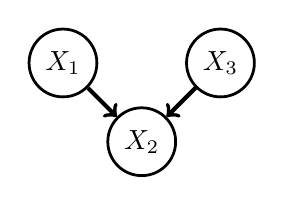
\begin{tikzpicture}[dgraph]
\node[cont] (A) at (0,1) {$X_1$};
\node[cont] (C) at (1,0) {$X_2$};
\node[cont] (B) at (2,1) {$X_3$};
\draw(A) -- (C);\draw(B) -- (C);
\end{tikzpicture}}
\end{center}
$$p(x_1,x_2,x_3) = p(x_2\mid x_1, x_3)p(x_3)p(x_1)$$
\bmp{0.5\tw}
\begin{center}
\begin{tabular}{ccc|c}
$x_2$ & $x_1$ & $x_3$ & $ p(x_2\mid x_3,x_1)$\\ \hline  0 & 0 & 0 & $\theta_1$\\ 0 & 0 & 1& $\theta_2$ \\  0 & 1 & 0 & $\theta_3$ \\  0 & 1 & 1 & $\theta_4$ \\ 
 1 & 0 & 0 & $1 - \theta_1$\\1 & 0 & 1& $1- \theta_2$ \\ 1 & 1 & 0 & $1-\theta_3$ \\ 1 & 1 & 1 & $1-\theta_4$ \\ 
\end{tabular}
\end{center}
\emp
\bmp{0.5\tw}
\begin{center}
\begin{tabular}{c|c}
$x_1$ & $p(x_1)$ \\ \hline  0 & $\theta_5$\\  1 & $1-\theta_5$  \\
\end{tabular}
\end{center}
\begin{center}
\begin{tabular}{c|c}
$x_3$ & $p(x_3)$ \\ \hline  0 & $\theta_6$\\  1 & $1-\theta_6$  \\ 
\end{tabular}
\end{center}
\emp
\end{mybox}
\vspace{0.5cm}
\item \textit{Bayesian Network Examples  }


Solution.
\vspace{0.5cm}

Draw the DAG associated with the following probability distributions:
	\begin{enumerate}
		\item $p(x_1,x_2,x_3) = p(x_2)p(x_3)p(x_2\mid x_1,x_3)$. Show that $X_1 \ci X_3 $.
\begin{center}
\scalebox{0.8}{
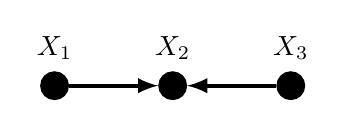
\begin{tikzpicture}[dgraph]
\node[contblk,label=above:{$X_1$}] (x1) at (0,0) {};
\node[contblk, label=above:{$X_2$}] (x2) at (1.5, 0) {};
\node[contblk, label=above:{$X_3$}] (x3) at (3,-0) {};
\draw [-{latex[slant=0]}]  (x1) -- (x2);
\draw [-{latex[slant=0]}] (x3) -- (x2);
\end{tikzpicture}}
\end{center}	
		\item $p(x_1,x_2,x_3) = p(x_1)p(x_2|x_1)p(x_3|x_2)$. Show that $X_1 \ci X_3 | X_2$.		
\begin{center}
\scalebox{0.8}{
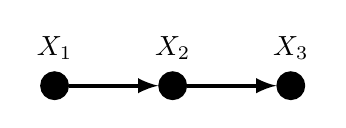
\begin{tikzpicture}[dgraph]
\node[contblk,label=above:{$X_1$}] (x1) at (0,0) {};
\node[contblk, label=above:{$X_2$}] (x2) at (1.5, 0) {};
\node[contblk, label=above:{$X_3$}] (x3) at (3,-0) {};
\draw [-{latex[slant=0]}]  (x1) -- (x2);
\draw [-{latex[slant=0]}] (x2) -- (x3);
\end{tikzpicture}}
\begin{align*}
p(x_1,x_3\mid x_2) &= \frac{p(x_1,x_2,x_3)}{p(x_2)}\\
&= \frac{p(x_1)p(x_2|x_1)p(x_3|x_2)}{p(x_2)}\\
&= \frac{p(x_1,x_2)p(x_3|x_2)}{p(x_2)}\\
&= \frac{p(x_1\mid x_2)p(x_2)p(x_3|x_2)}{p(x_2)}\\
&= p(x_1|x_2)p(x_3|x_2)\\ & \Longrightarrow X_1 \ci X_3 | X_2
\end{align*}
\end{center}		
		\item $p(x_1,x_2,x_3) = p(x_2)p(x_1|x_2)p(x_3|x_2)$. Show that $X_1\ci X_3 | X_2$.		
\begin{center}
\scalebox{0.8}{
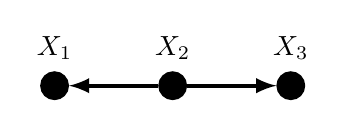
\begin{tikzpicture}[dgraph]
\node[contblk,label=above:{$X_1$}] (x1) at (0,0) {};
\node[contblk, label=above:{$X_2$}] (x2) at (1.5, 0) {};
\node[contblk, label=above:{$X_3$}] (x3) at (3,-0) {};
\draw [-{latex[slant=0]}]  (x2) -- (x1);
\draw [-{latex[slant=0]}] (x2) -- (x3);
\end{tikzpicture}}
\end{center}
\begin{align*}
p(x_1,x_3\mid x_2) &= \frac{p(x_1,x_2,x_3)}{p(x_2)}\\
&= \frac{p(x_2)p(x_1|x_2)p(x_3|x_2)}{p(x_2)}\\
&= p(x_1|x_2)p(x_3|x_2)\\ & \Longrightarrow X_1 \ci X_3 | X_2
\end{align*}		
		\item $p(x_1,x_2,x_3,x_4) = p(x_1)p(x_2)p(x_3|x_1)p(x_4|x_1,x_2)$. Show that $X_3 \ci X_4 | X_1$.
\begin{center}
\scalebox{0.8}{
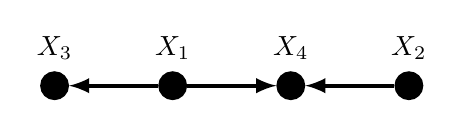
\begin{tikzpicture}[dgraph]
\node[contblk,label=above:{$X_3$}] (x3) at (0,0) {};
\node[contblk, label=above:{$X_1$}] (x1) at (1.5, 0) {};
\node[contblk, label=above:{$X_4$}] (x4) at (3, -0) {};
\node[contblk, label=above:{$X_2$}] (x2) at (4.5,-0) {};
\draw [-{latex[slant=0]}]  (x1) -- (x3);
\draw [-{latex[slant=0]}] (x1) -- (x4);
\draw [-{latex[slant=0]}]  (x2) -- (x4);
\end{tikzpicture}}
\end{center}		
		\item $p(x_1,x_2,x_3,x_4,x_5) = p(x_1)p(x_2)p(x_3|x_1)p(x_4|x_1,x_2)p(x_5|x_4)$. Show that $X_1 \ci X_5 | X_4$.
\begin{center}
\scalebox{0.8}{
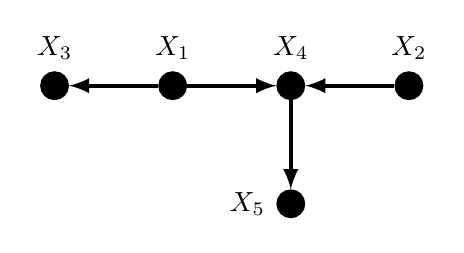
\begin{tikzpicture}[dgraph]
\node[contblk,label=above:{$X_3$}] (x3) at (0,0) {};
\node[contblk, label=above:{$X_1$}] (x1) at (1.5, 0) {};
\node[contblk, label=above:{$X_4$}] (x4) at (3, -0) {};
\node[contblk, label=above:{$X_2$}] (x2) at (4.5,-0) {};
\node[contblk, label=left:{$X_5$}] (x5) at (3,-1.5) {};
\draw [-{latex[slant=0]}]  (x1) -- (x3);
\draw [-{latex[slant=0]}] (x1) -- (x4);
\draw [-{latex[slant=0]}]  (x2) -- (x4);
\draw [-{latex[slant=0]}]  (x4) -- (x5);
\end{tikzpicture}}
\end{center}		
		\item $p(x_1,x_2,x_3,x_4,x_5,x_6) = p(x_1)p(x_2|x_1)p(x_3|x_1)p(x_4|x_2)p(x_5|x_3)p(x_6|x_2,x_5).$ Show that $X_2 \ci X_3 | X_1$.
\begin{center}
\scalebox{0.8}{
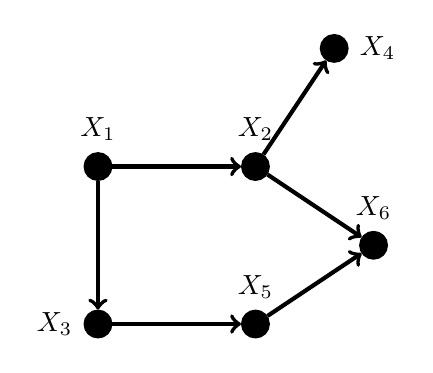
\begin{tikzpicture}[dgraph]
\node[contblk,label=above:{$X_1$}] (x1) at (0,0) {};
\node[contblk,label=above:{$X_2$}] (x2) at (2, 0) {};
\node[contblk,label=left:{$X_3$}] (x3) at (0,-2) {};
\node[contblk,label=right:{$X_4$}] (x4) at (3,1.5) {};
\node[contblk,label=above:{$X_5$}] (x5) at (2,-2) {};
\node[contblk,label=above:{$X_6$}] (x6) at (3.5,-1) {};
\draw(x1) -- (x2);
\draw(x1) -- (x3);
\draw(x2) -- (x4);
\draw(x3) -- (x5);
\draw(x2) -- (x6);
\draw(x5) -- (x6);
\end{tikzpicture}}
\end{center}	

\item Write down the factorization of $p(x_1,x_2,x_3,x_4,x_5,x_6,x_7) $ encoded in the following DAG.
\begin{center}
\scalebox{.9}{
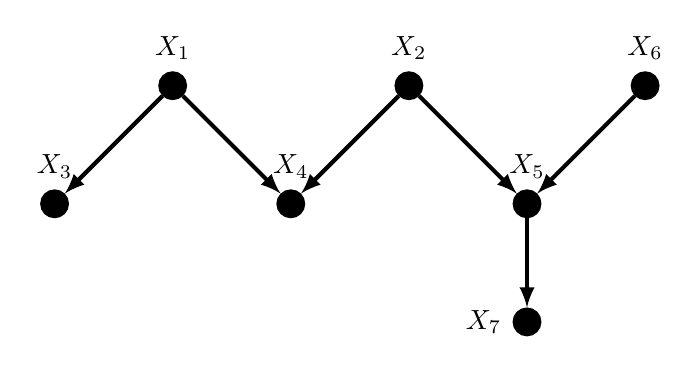
\begin{tikzpicture}[dgraph]
\node[contblk,label=above:{$X_3$}] (x3) at (0,0) {};
\node[contblk, label=above:{$X_1$}] (x1) at (1.5, 1.5) {};
\node[contblk, label=above:{$X_4$}] (x4) at (3, -0) {};
\node[contblk, label=above:{$X_2$}] (x2) at (4.5,1.5) {};
\node[contblk, label=above:{$X_5$}] (x5) at (6, -0) {};
\node[contblk, label=left:{$X_7$}] (x7) at (6, -1.5) {};
\node[contblk, label=above:{$X_6$}] (x6) at (7.5,1.5) {};

\draw [-{latex[slant=0]}]  (x1) -- (x3);
\draw [-{latex[slant=0]}] (x1) -- (x4);
\draw [-{latex[slant=0]}]  (x2) -- (x4);
\draw [-{latex[slant=0]}]  (x2) -- (x5);
\draw [-{latex[slant=0]}]  (x6) -- (x5);
\draw [-{latex[slant=0]}]  (x5) -- (x7);
\end{tikzpicture}}
\end{center}

	\end{enumerate}

\end{itemize}




\begin{mybox}{Application Example (Was it the burglar?) }{theoexample}
 Mary lives in San Francisco City. One afternoon, she is driving back home and receives a phone call from 
 her neighbor Jane. She told her that her house alarm was set off ($\mathsf  A$). While driving, she also heard on the radio
 ($\mathsf  R$) that a small earthquake ($\mathsf  E$) hit the city.  Small earthquakes sometimes activate the alarm, and perhaps
 this is the reason why the alarm was sounding.
 \begin{itemize}
 \item What is the probability that a burglar ($\mathsf B$) broke into the house?
 \item What is the probability that a burglar broke into the house
 given that the alarm was set off?
 \item What is the probability that a burglar broke into the house
 given that the alarm was set off and a small earthquake hit the city?
 \end{itemize} 
\end{mybox}

To solve this problem we make several considerations.
\begin{enumerate}
\item Define the random variables $R(\mathsf R )=1$, $R(\mathsf R^c )=0$, $A(\mathsf A )=1$, $A(\mathsf A^c )=0$,
$E(\mathsf E )=1$, $E(\mathsf E^c )=0$, and $B(\mathsf B )=1$, $B(\mathsf B^c )=0$.
\item Assume that the joint distribution of random variables $R$, $A$, $E$, and $B$ factorizes as 
 $$\small p(A,R,E,B)=p(E=e)p(B=b)p(A=a\mid B=b,E=e)p(R=r\mid E=e)$$ our using our simplified 
notation
 $$p(a,r,e,b)=p(e)p(b)p(a\mid b,e)p(r\mid e).$$
\end{enumerate}




The factors of the probability distribution correspond to the following tables.
 
  \bmp{0.4\tw}  
  \begin{center}
  \begin{tabular}{l l l }
    \hline
            & $b$ & $p(b)$ \\\hline\hline
     $\mathsf{B^c}$ & $\mathsf 0$ & $\mathsf{b_1 = .9}$\\
     $\mathsf{B}$    &  $\mathsf 1$ & $1-\mathsf{b_1}$\\     
     \hline
  \end{tabular}
  
  \vspace{0.2cm}
  \begin{tabular}{l l l }
    \hline
            & $e$ & $p(e)$ \\\hline\hline
     $\mathsf{E^c}$ & $\mathsf 0$ & $\mathsf{e_1 = 0.95}$\\
     $\mathsf{E}$    &  $\mathsf 1$ & $\mathsf{e_2=1-e_1}$ \\     
     \hline
  \end{tabular}
    \vspace{0.2cm}
%  \begin{tabular}{l l l }
%    \hline
%            & $r$ & $p(r)$ \\\hline\hline
%     $\mathsf{R^c}$ & $\mathsf 0$ & $\mathsf{c_1 = 0.05}$\\
%     $\mathsf{R}$    &  $\mathsf 1$ & $\mathsf{c_2=1-c_1}$\\     
%     \hline
%  \end{tabular}  
\end{center}
\emp
 \bmp{0.6\tw}  
  \begin{center}
  \begin{tabular}{l l l l l}
    \hline
                              &                           & $b$  & $e $ & $p(b,e)$ \\\hline\hline
     $\mathsf{B^c}$ &  $\mathsf{E^c}$ &  $\mathsf 0$     &   $\mathsf 0$    &  $\mathsf{b_1e_1}$\\
     $\mathsf{B^c}$ &  $\mathsf{E}$    &  $\mathsf 0$     &   $\mathsf 1$    &  $\mathsf{b_1e_2}$\\  
     $\mathsf{B}$    &  $\mathsf{E^c}$ &  $\mathsf 1$     &   $\mathsf 0$    &  $\mathsf{b_2e_1}$\\
     $\mathsf{B}$.   &  $\mathsf{E}$    &  $\mathsf 1$        &   $\mathsf 1$    &  $\mathsf{b_2e_2}$\\     
        
     \hline
  \end{tabular}
\end{center}
  \begin{center}
  \begin{tabular}{l l l l l}
    \hline
                              &                           & $r$  & $e $ & $p(r\mid e)$ \\\hline\hline
     $\mathsf{R^c}$ &  $\mathsf{E^c}$ &  $\mathsf 0$     &   $\mathsf 0$    &  $\mathsf f_1=0.99$\\
     $\mathsf{R^c}$ &  $\mathsf{E}$    &  $\mathsf 0$     &   $\mathsf 1$    &  $\mathsf f_2=0.01$\\  
     $\mathsf{R}$    &  $\mathsf{E^c}$ &  $\mathsf 1$     &   $\mathsf 0$    &  $\mathsf{f_3=1-f_1}$\\
     $\mathsf{R}$.   &  $\mathsf{E}$    &  $\mathsf 1$        &   $\mathsf 1$    &  $\mathsf {f_4=1-f_2}$\\     
        
     \hline
  \end{tabular}
\end{center}
\emp
\vspace{0.5cm}

   \bmp{0.6\tw}  
  \begin{center}
  \begin{tabular}{l l l l  l l l l l }
    \hline
               &       &     &  $ { a}$ & $ { b}$ & $ { e}$ &$ p(a\mid b,e)$ \\ \hline\hline
     $\mathsf{A^c}$ & $\mathsf{B^c}$ & $\mathsf{E^c}$   & $ \mathsf{ 0}$ & $\mathsf {0}$ & $  \mathsf {0}$ &$ \mathsf{q_1}$ \\ %\hline
     $\mathsf{A^c}$ & $\mathsf{B^c}$ & $\mathsf{E}$    & $ \mathsf{0}$ & $\mathsf {0}$ & $  \mathsf {1}$ &  $  \mathsf{q_2}$ \\ %\hline
     $\mathsf{A^c}$ & $\mathsf{B}$ & $\mathsf{E^c}$     & $\mathsf{ 0}$ & $\mathsf {1}$ & $ \mathsf {0}$ &  $ \mathsf{q_3}$ \\ %\hline
     $\mathsf{A^c}$ & $\mathsf{B}$ & $\mathsf{E}$    & $ \mathsf{ 0}$ & $\mathsf{1}$ & $  \mathsf{1}$ &  $ \mathsf{q_4}$ \\ %\hline
     $\mathsf{A}$ & $\mathsf{B^c}$ & $\mathsf{E^c}$     & $ \mathsf{ 1}$ & $\mathsf {0}$ & $  \mathsf {0}$ &  $  \mathsf{q_5=1-q_1}$\\ %\hline
     $\mathsf{A}$ & $\mathsf{B^c}$ & $\mathsf{E}$    & $ \mathsf{ 1}$ & $\mathsf {0}$ & $  \mathsf{1}$ &  $ \mathsf{q_6=1-q_2}$ \\ %\hline
     $\mathsf{A}$ & $\mathsf{B}$ & $\mathsf{E^c}$     & $ \mathsf{ 1}$ & $\mathsf{1}$ & $ \mathsf {0}$ &  $  \mathsf{q_7=1-q_3}$ \\ %\hline
     $\mathsf{A}$ & $\mathsf{B}$ & $\mathsf{E}$     & $ \mathsf{ 1}$ & $\mathsf{1}$ & $  \mathsf{1}$ &  $  \mathsf{q_8=1-q_4}$ \\ %\hline
    \hline
  \end{tabular}
\end{center}
\emp
\bmp{0.4\tw}  
  \begin{center}
  


\end{center}
\emp

\vspace{0.5cm}

The table representing the joint probability function is 
\vspace{0.5cm}

   \bmp{0.7\tw}  
  \begin{center}
  \begin{tabular}{l l l l  l l l l l }
    \hline
        &       &       &     &  $ {  a}$ & $ { r}$ & $ { b}$ & $ { e}$ &$ p(r,a,e,b)$ \\ \hline\hline
   $\mathsf{A^c}$ & $\mathsf{R^c}$ & $\mathsf{B^c}$ & $\mathsf{E^c}$ &  $ \mathsf{ 0}$ & $ \mathsf{ 0}$ & $\mathsf {0}$ & $  \mathsf {0}$ &$ \mathsf{p_1}=     \mathsf{b_1e_1f_1q_1}$ \\ %\hline
   $\mathsf{A^c}$ & $\mathsf{R^c}$ & $\mathsf{B^c}$ & $\mathsf{E}$ &  $ \mathsf{ 0}$  & $ \mathsf{0}$ & $\mathsf {0}$ & $  \mathsf {1}$ &  $  \mathsf{p_2}=    \mathsf{b_2e_1f_1q_1}$ \\ %\hline
   $\mathsf{A^c}$ & $\mathsf{R^c}$ & $\mathsf{B}$ & $\mathsf{E^c}$ &  $ \mathsf{ 0}$  & $\mathsf{ 0}$ & $\mathsf {1}$ & $ \mathsf {0}$ &  $ \mathsf{p_3}=     \mathsf{b_1e_2f_2q_2}$ \\ %\hline
   $\mathsf{A^c}$ & $\mathsf{R^c}$ & $\mathsf{B}$ & $\mathsf{E}$ &  $\mathsf{ 0}$  & $ \mathsf{ 0}$ & $\mathsf{1}$ & $  \mathsf{1}$ &  $ \mathsf{p_4}=      \mathsf{b_2e_2f_2q_2}$ \\ %\hline
   $\mathsf{A^c}$ & $\mathsf{R}$ & $\mathsf{B^c}$ & $\mathsf{E^c}$ &  $\mathsf{ 0}$  & $ \mathsf{ 1}$ & $\mathsf {0}$ & $  \mathsf {0}$ &  $  \mathsf{p_5}=     \mathsf{b_1e_1f_3q_3}$\\ %\hline
   $\mathsf{A^c}$ & $\mathsf{R}$ & $\mathsf{B^c}$ & $\mathsf{E}$ &  $\mathsf{ 0}$  & $ \mathsf{ 1}$ & $\mathsf {0}$ & $  \mathsf{1}$ &  $ \mathsf{p_6}=     \mathsf{b_2e_1f_3q_3}$ \\ %\hline
   $\mathsf{A^c}$ & $\mathsf{R}$ & $\mathsf{B}$ & $\mathsf{E^c}$ &  $\mathsf{ 0}$  & $ \mathsf{ 1}$ & $\mathsf{1}$ & $ \mathsf {0}$ &  $  \mathsf{p_7}=      \mathsf{b_1e_2f_4q_4}$ \\ %\hline
   $\mathsf{A^c}$ & $\mathsf{R}$ & $\mathsf{B}$ & $\mathsf{E}$ &  $\mathsf{0}$   & $ \mathsf{ 1}$ & $\mathsf{1}$ & $  \mathsf{1}$ &  $  \mathsf{p_8}=       \mathsf{b_2e_2f_4q_4}$ \\ %\hline
   $\mathsf{A}$ & $\mathsf{R^c}$ & $\mathsf{B^c}$ & $\mathsf{E^c}$ &  $ \mathsf{1}$  & $ \mathsf{ 0}$ & $\mathsf {0}$ & $ \mathsf {0}$ &  $ \mathsf{p_9}=     \mathsf{b_1e_1f_1q_5}$ \\ %\hline
   $\mathsf{A}$ & $\mathsf{R^c}$ & $\mathsf{B^c}$ & $\mathsf{E}$ &  $\mathsf{ 1}$  & $ \mathsf{ 0}$ & $\mathsf {0}$ & $  \mathsf{1}$ &  $  \mathsf{p_{10}}= \mathsf{b_2e_1f_1q_5}$ \\ %\hline
   $\mathsf{A}$ & $\mathsf{R^c}$ & $\mathsf{B}$ & $\mathsf{E^c}$ &  $\mathsf{ 1}$  & $ \mathsf{ 0}$ & $\mathsf{1}$ & $ \mathsf {0}$ &  $  \mathsf{p_{11}}=  \mathsf{b_1e_2f_2q_6}$ \\ %\hline
   $\mathsf{A}$ & $\mathsf{R^c}$ & $\mathsf{B}$ & $\mathsf{E}$ &  $\mathsf{ 1}$  & $ \mathsf{ 0}$ & $\mathsf{1}$ & $ \mathsf {1}$ &  $  \mathsf{p_{12}}=  \mathsf{b_2e_2f_2q_6}$ \\ %\hline
   $\mathsf{A}$ & $\mathsf{R}$ & $\mathsf{B^c}$ & $\mathsf{E^c}$ &  $\mathsf{ 1}$  & $ \mathsf{ 1}$ & $\mathsf{0}$ & $ \mathsf {0}$ &  $ \mathsf{p_{13}}=  \mathsf{b_1e_1f_3q_7}$ \\ %\hline
   $\mathsf{A}$ & $\mathsf{R}$ & $\mathsf{B^c}$ & $\mathsf{E}$ &  $\mathsf{ 1}$  & $ \mathsf{ 1}$ & $\mathsf{0}$ & $ \mathsf {1}$ &  $  \mathsf{p_{14}}=  \mathsf{b_2e_1f_3q_7}$ \\ %\hline
   $\mathsf{A}$ & $\mathsf{R}$ & $\mathsf{B}$ & $\mathsf{E^c}$ &  $\mathsf{ 1}$  & $ \mathsf{ 1}$ & $\mathsf{1}$ & $ \mathsf {0}$ &  $ \mathsf{p_{15}}=  \mathsf{b_1e_2f_4q_8}$ \\ %\hline
   $\mathsf{A}$ & $\mathsf{R}$ & $\mathsf{B}$ & $\mathsf{E}$ &  $\mathsf{ 1}$  & $ \mathsf{ 1}$ & $\mathsf{1}$ & $ \mathsf {1}$ &  $  \mathsf{p_{16}}=  \mathsf{b_2e_2f_4q_8}$ \\ %\hline

    \hline
  \end{tabular}
\end{center}
\emp
\bmp{0.3\tw}  
  \begin{center}
  
\end{center}
\emp  

\begin{marginfigure}
\centering
\begin{center}
\scalebox{.9}{
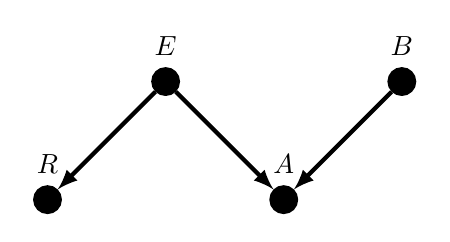
\begin{tikzpicture}[dgraph]
\node[contblk,label=above:{$R$}] (x3) at (0,0) {};
\node[contblk, label=above:{$E$}] (x1) at (1.5, 1.5) {};
\node[contblk, label=above:{$A$}] (x4) at (3, -0) {};
\node[contblk, label=above:{$B$}] (x2) at (4.5,1.5) {};
\draw [-{latex[slant=0]}]  (x1) -- (x3);
\draw [-{latex[slant=0]}] (x1) -- (x4);
\draw [-{latex[slant=0]}]  (x2) -- (x4);
\end{tikzpicture}}
\end{center}
\caption{Directed Acyclic Graph encoding the 
probability distribution $p(a,r,e,b)=p(e)p(b)p(a\mid b,e)p(r\mid e).$ Dark circles represent random variables $R$, $A$, $E$, and $B$. 
}

\end{marginfigure}

\vspace{0.5cm}

\begin{itemize}
\item The \textit{graphical model}  (a Directed Acyclic Graph or DAG) encoding the 
probability distribution factorization is shown in Figure 21.
\item Assume that  $q_1=0.98$, $q_2=0.9$, $q_3=0.1$, $q_4=0.01$.
\item What is the probability that a burglar broke into the house?
\begin{align*}
P(B=\mathsf 1) &= P(\mathsf{B}) = \\ &= \mathsf{ p_3+p_4+p_7+p_8+p_{11}+p_{12}+p_{15}+p_{16},}
\end{align*}
\begin{align*}
P(B=\mathsf 1) &= \sum_{a}\sum_{r}\sum_{e} p(r,a,B=1,e) = 0.1.
\end{align*}
%\item What is the computational complexity of computing $p(B)$?
\end{itemize}

\begin{itemize}
\item What is the probability that a burglar broke into the house
 given that the alarm was set off?
\begin{align*}
P(B=\mathsf 1\mid A=1) &= \frac{P(B=1,A=1 )}{P(A=1)}\\ &= \frac{\mathsf{ p_{11}+p_{12}+p_{15}+p_{16}}}{\mathsf{p_{9}+p_{10}+p_{11}+p_{12}+p_{13}+p_{14}+p_{15}+p_{16}}},
\end{align*}
\begin{align*}
P(B=\mathsf 1\mid A=1) &= \frac{\sum_{r}\sum_{e} p(r,A=1,B=1,e)}{\sum_{r}\sum_{b}\sum_{e} p(r,A=1,b,e) } &= 0.81.
\end{align*}
\end{itemize}

\begin{itemize}
\item What is the probability that a burglar broke into the house
 given that the alarm was set off and a small earthquake hit the city?
\begin{align*}
P(B=\mathsf 1\mid A=1, E=1) &= \frac{P(B=1,A=1,E=1 )}{P(A=1,E=1)}\\ &= \frac{\mathsf{p_{12} +p_{16}}}{\mathsf{p_{10}+ p_{12}+p_{14}+p_{16}}},
\end{align*}
\begin{align*}
P(B=\mathsf 1\mid A=1,E=1) &= \frac{\sum_{r}p(r,A=1,B=1,E=1)}{\sum_{r}\sum_{b} p(r,A=1,b,E=1) } \\&= 0.51.
\end{align*}
\end{itemize}

\begin{mybox}{Solution Summary }{theoexample}
\begin{itemize}
 \item What is the probability that a burglar broke into the house?
 \begin{align*}
P(B=\mathsf 1) &= 0.1.
\end{align*}
 \item What is the probability that a burglar broke into the house
 given that the alarm was set off?
 \begin{align*}
P(B=\mathsf 1\mid A=1) &= 0.81.
\end{align*}
 \item What is the probability that a burglar broke into the house given that the alarm was set off and a small earthquake hit the city?
 \begin{align*}
P(B=\mathsf 1\mid A=1,E=1) &= 0.51.
\end{align*}
\item The \textit{a priori} probability that the burglar broke into the house is $0.1$. The probability that a burglar broke into the house
 given that the alarm was set off is much higher  ($0.81$). However, knowing that a small earthquake hit the city \textit{explains away} the observation that the alarm was set off,
 diminishing the probability that a burglar broke ($0.51$). 
 \end{itemize} 
\end{mybox}
\begin{itemize}
 \item Note that the factorization features of the probability distribution and the sum-product distributive property help us reduce the computational complexity. 
 \begin{align*}
 p(b\mid a) = \frac{p(a,b)}{p(a)} &= \frac{\sum_r\sum_ep(r,a,e,b)}{\sum_b\sum_r\sum_ep(r,a,e,b)}\\
 					       &= \frac{\sum_r\sum_e p(e)p(b)p(a\mid e,b)p(r\mid e)}{\sum_b\sum_r\sum_e p(e)p(b)p(a\mid e,b)p(r\mid e)}\\
                                                 &= \frac{p(b)\sum_e p(e)p(a\mid e,b)\sum_rp(r\mid e)}{\sum_bp(b)\sum_e p(e)p(a\mid e,b)\sum_rp(r\mid e)}\\
                                                 &= \frac{p(b)\sum_e p(e)p(a\mid e,b)\phi_1(e)}{\sum_b p(b)\sum_e p(e)p(a\mid e,b)\phi_1(e)}\\
                                                  &= \frac{p(b)\phi_2(a,b)}{\sum_b p(b)\phi_2(a,b)}\\
                                                 &= \frac{p(b)\phi_2(a,b)}{\phi_3(a)}\\
 \end{align*}
\end{itemize}

\begin{mybox}{Application Example (Pairs of dice) }{theoexample}
\small
You are told that there are two pairs of coins. The first pair is fair, $$\theta_1(\mathsf H)=\theta_1(\mathsf T)=\frac{1}{2}.$$ The second pair is biased as both coins have probability $$\theta_2(\mathsf H)=\frac{2}{3},\,\, \theta_2(\mathsf T)=\frac{1}{3}$$  of producing heads  and  tails, respectively. One of the two pairs is chosen at random with probability 0.5 and thrown 10 times. The sum of the coins is recorded for each throw.
 \begin{enumerate}
\item If the throw results in the sequence "1010101010"? Which pair of dice was picked for the throw?
\item Repeat (1) for the sequence "2222200000". 
\item Assume that the result of the second coin is flipped ($\mathsf F$) with probability $\sf p=0.5$ before recording the result of the throw with probability. Repeat  1 and 2 under this assumption. Consider the case for which  $\sf p = 0.2$. Repeat exercises 1 and 2.
\vspace{0.2cm}

\noindent The graphical model associated with this problem is as follows.

\begin{center}
\scalebox{0.8}{
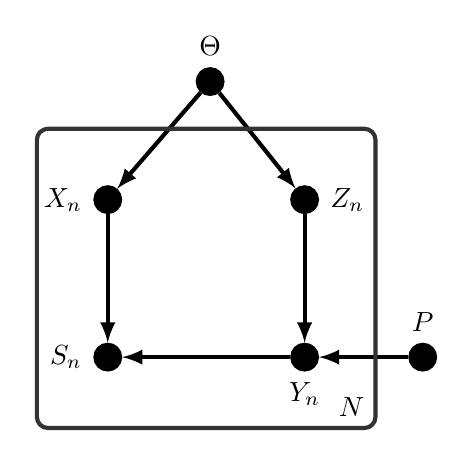
\begin{tikzpicture}[dgraph]
\node[contblk,label=above:{$\Theta$}] (theta) at (2.3,1.5) {};
\node[contblk, label=left:{$X_n$}] (xn) at (1, 0) {};
\node[contblk, label=right:{$Z_n$}] (zn) at (3.5, 0) {};
\node[contblk, label=below:{$Y_n$}] (yn) at (3.5,-2) {};
\node[contblk, label=left:{$S_n$}] (sn) at (1,-2) {};
\node[contblk, label=above:{$P$}] (p) at (5.0,-2) {};
\draw [-{latex[slant=0]}]  (theta) -- (xn);
\draw [-{latex[slant=0]}] (theta) -- (zn);
\draw [-{latex[slant=0]}]  (zn) -- (yn);
\draw [-{latex[slant=0]}]  (xn) -- (sn);
\draw [-{latex[slant=0]}]  (yn) -- (sn);
\draw [-{latex[slant=0]}]  (p) -- (yn);
\boxit{$N$}{(sn)}{(zn)}{0.9};
\end{tikzpicture}}
\end{center}
\end{enumerate}
\begin{itemize}
\item $X_n$ represents the $n$-th result from the throw of the first coin; $X_n(\sf H) = 1$ and $X_n(\sf T) = 0$, and
$$p(x_n\mid \theta) = \theta^{x_n}(1-\theta)^{(1-x_n)}. $$ 
\item $Z_n$ epresents the unobserved   result from the $n$-th throw of the second coin;  $Z_n(\sf F) = 1$ and $Z_n(\sf F^c) = 0$, and
$$p(z_n\mid \theta) = \theta^{z_n}(1-\theta)^{(1-z_n)}. $$
\item $Y_n$ represents the recorded result  from the $n$-th throw of the second coin; $Y_n(\sf H) = 1$ and $Y_n(\sf T) = 0$, and 
$$p(y_n\mid z_n, p) = p^{I(y_n \neq z_n)} (1-p)^{ I(y_n = z_n)}.$$
\item $S_n$ is a deterministic function of $X_n$ and $Y_n$,  $$S_n=X_n+Y_n,$$ $$p(s_n\mid x_n, y_n) = \mathrm I(s_n == x_n+y_n),$$ and
\begin{equation*}
 I(e) =
    \begin{cases}
      1, & \textrm{if}\,\,e = \mathsf{true};\\
      0, & \textrm{otherwise}.\\
    \end{cases}       
\end{equation*}
 
\end{itemize}
\end{mybox}

Let  $\mathbf X = (X_1,X_2, \dots, X_N)$,  $\mathbf Y = (Y_1,Y_2, \dots, Y_N)$,  $\mathbf Z = (Z_1,Z_2, \dots, Z_N)$,
$\mathbf S = (S_1,S_2, \dots, S_N)$, $f_n= I(y_n \neq z_n) = 1 - I(y_n = z_n)$, and $\mathbf f = (f_1,f_2, \dots, f_N)$. ($f_n$ indicates whether the second was flipped or not.) 
The joint probability distribution for  $\mathbf x, \mathbf z, \mathbf y, \mathbf s $ given $\theta$ and $p$ is

\begin{align*}
p(\mathbf x, \mathbf z, \mathbf y, \mathbf s, \theta,  p) &= p(\theta)p(p)\prod_{n=1}^{N} p(x_n\mid \theta)p(z_n\mid \theta)p(y_n\mid z_n, p) p(s_n \mid x_n,y_n)\\
p(\mathbf x, \mathbf z, \mathbf y, \mathbf s \mid \theta,  p) &= \frac{p(\mathbf x, \mathbf z, \mathbf y, \mathbf s, \theta,  p)}{p(\theta)p(p)}\\
p(\mathbf x, \mathbf z, \mathbf y, \mathbf s \mid \theta,  p)  &= \prod_{n=1}^{N} p(x_n\mid \theta)p(z_n\mid \theta)p(y_n\mid z_n, p) p(s_n \mid x_n,y_n)\\
&=  \prod_{n=1}^{N}  \theta^{x_n}(1-\theta)^{(1-x_n)}  \theta^{z_n}(1-\theta)^{(1-z_n)} p^{I(y_n \neq z_n)} (1-p)^{ I(y_n = z_n)}  I(s_n = x_n + y_n).\\
&=  \theta^{\sum_{n=1}^N x_n}(1-\theta)^{\sum_{n=1}^N(1-x_n)}  \theta^{\sum_{n=1}^N z_n}(1-\theta)^{\sum_{n=1}^N(1-z_n)} p^{\sum_{n=1}^N I(y_n \neq z_n)} (1-p)^{ \sum_{n=1}^N I(y_n = z_n)} \\
\end{align*}

Notice that 

$$x_n = s_n - y_n,$$
$$y_n = z_n(1-f_n)+(1-z_n)f_n,$$ and
$$x_n = s_n - z_n + 2z_nf_n - f_n.$$

We define $N_x$, and $N_z$ as follows,

$$ N_x = \sum_{n=1}^{N} (s_n - z_n + 2z_nf_n - f_n) = N_s - N_z + 2N_{zf}-N_f  \geq 0,$$
$$ N_s = \sum_{n=1}^{N} s_n,$$
$$ N_z = \sum_{n=1}^{N} z_n,$$
$$ N_{zf} = \sum_{n=1}^{N} z_nf_n,$$and
$$N_f = \sum_{n=1}^{N} f_n.$$

Therefore we can write the probability distribution function as follows,
\begin{align*}
p(\mathbf x, \mathbf z, \mathbf y, \mathbf s \mid \theta,  p) &=  \theta^{\sum_{n=1}^N x_n}(1-\theta)^{\sum_{n=1}^N(1-x_n)}  \theta^{\sum_{n=1}^N z_n}(1-\theta)^{\sum_{n=1}^N(1-z_n)} p^{\sum_{n=1}^N f_n} (1-p)^{ \sum_{n=1}^N (1-f_n)} \\
&=  \theta^{N_x}(1-\theta)^{(N-N_x)} \theta^{N_z}(1-\theta)^{(N-N_z)}p^{N_f}(1-p)^{N-N_f}\\
&=  \theta^{N_x + N_z }(1-\theta)^{(2N-(N_x+N_z))} p^{N_f}(1-p)^{N-N_f}\\
&= p(\mathbf s, \mathbf z, \mathbf f \mid \theta, p)
\end{align*}
Observe  that 
$N_x = N_x(\mathbf s,\mathbf z, \mathbf f),$
$N_z = N_z(\mathbf z),$ and therefore

$$ p(\mathbf x, \mathbf z, \mathbf y, \mathbf s \mid \theta, p) =  p(\mathbf s, \mathbf z, \mathbf f \mid \theta, p). $$  Also,

$$ p(\mathbf s \mid \theta, p) =  \sum_{\mathbf x}  \sum_{\mathbf z} \sum_{\mathbf y} p(\mathbf x, \mathbf z, \mathbf y, \mathbf s \mid \theta, p) =  \sum_{\mathbf f} \sum_{\mathbf z} p(\mathbf s, \mathbf z, \mathbf f \mid \theta, p),$$ and

\begin{align*}
p(\theta\mid \mathbf s, p) &= \frac{p(\mathbf s, \theta, p)}{p( \mathbf s, p)}= \frac{p(\mathbf s\mid \theta, p)p(\theta,p)}{p( \mathbf s, p)} \\
                                         &=  \frac{p(\mathbf s\mid \theta, p)p(\theta\mid p)p(p)}{p( \mathbf s\mid p)p(p)}\\
                                         &=  \frac{p(\mathbf s\mid \theta, p)p(\theta\mid p)}{p( \mathbf s\mid p)}\\
                                         &=  \frac{p(\mathbf s\mid \theta, p)p(\theta)}{p( \mathbf s\mid p)}. 
\end{align*}
since $\theta \ci p$.

 \begin{mybox}{Decision Rule }{theoexample}

$$ \mathrm I\left(\frac{p(\theta_1 \mid ,\mathbf s,  p)}  {p(\theta_2 \mid ,\mathbf s,  p)} > 1 \right)  \Rightarrow \text{choose $ \theta_1$},$$ 
which is equivalent to
$$ \mathrm I\left(\frac{p(\mathbf s \mid \theta_1, p)p(\theta_1)}  {p(\mathbf s \mid \theta_2, p)p(\theta_2)} > 1 \right)  \Rightarrow \text{choose $ \theta_1$},$$ 
since
$$p(\theta \mid ,\mathbf s,  p) \propto  p(\mathbf s \mid \theta, p)p(\theta) =    \sum_{\mathbf f} \sum_{\mathbf z} p(\mathbf s, \mathbf z, \mathbf f \mid \theta, p) p(\theta).$$

Notice that 

$$ p(\mathbf s|p) = \sum_{\theta} \sum_{\mathbf f} \sum_{\mathbf z} p(\mathbf s, \mathbf z, \mathbf f \mid \theta, p)p(\theta),$$ with $\theta \in \{\theta_1,\theta_2\}.$

\end{mybox}

\begin{marginfigure}
\centering
\includegraphics[width=4cm]{fig/12.png}
\caption{Probability distribution $p(N_s)$ in Box for $\theta= \frac{1}{2}$ for problem 3 in Box 9.
The expected value $\mu_{N_s}= 5$ and the entropy is $E(N_s)=2.71$.
}
\end{marginfigure}




These equations lead to the following results regarding question 3.

\begin{align*}
\frac{p([2, 2, 2, 2, 2, 0, 0, 0, 0, 0]\mid \frac{2}{3}, \frac{1}{2})p(\frac{2}{3})}{p([2, 2, 2, 2, 2, 0, 0, 0, 0, 0]\mid  \frac{1}{2}, \frac{1}{2})p(\frac{1}{2})} &= 1.80 \Longrightarrow  \theta_2 = \frac{2}{3}.\\
\frac{p([1,0,1,0,1,0,1,0,1,0]\mid \frac{2}{3}, \frac{1}{2})p(\frac{2}{3})}{p([1,0,1,0,1,0,1,0,1,0]\mid  \frac{1}{2}, \frac{1}{2})p(\frac{1}{2})} &= 0.13 \Longrightarrow  \theta_1 = \frac{1}{2}. 
\end{align*}

\begin{figure}
\centering
\includegraphics[width=3.8cm]{fig/1-99.100.png}\includegraphics[width=3.8cm]{fig/1-8.9.png}\includegraphics[width=3.8cm]{fig/1-4.5.png}

\includegraphics[width=3.8cm]{fig/4.5.png}\includegraphics[width=3.8cm]{fig/8.9.png}\includegraphics[width=3.8cm]{fig/99.100.png}
\caption{From left to right and from top to bottom, probability distributions $p(N_s)$ in Box for $\theta= \frac{1}{100}$,  $\theta$ are $\frac{1}{9}$, $ \frac{1}{5}$, $ \frac{99}{100}$,  $\frac{8}{9}$, $\frac{4}{5}$ for problem 3 in Box 9. The corresponding mean values, $\mu_{N_s}$, are $2.55$, $3.06$, $3.5$, $6.5$, $6.9$, respectively.
and $\mu_{N_s}=7.45$, respectively. The corrresponding entropies, $E(N_s)$, are $2.44$,  $2.56$,  $2.56$,  $2.44$, and  $2.22$, respectively. 
}
\end{figure}


Also, notice that
\begin{align*}
\mathrm E[\mathbf s\mid \theta, p] &=  \sum_{\mathbf s} \sum_{\mathbf f} \sum_{\mathbf z} \mathbf s p(\mathbf s, \mathbf z, \mathbf f \mid \theta, p),\\ 
\mathrm E[N_s\mid \theta, p] &=   \sum_{N_s}  N_s p(N_s\mid \theta, p).
\end{align*}
The  \textit{effect} of $\theta$ on $N_s$ is
\begin{align*}
e(\theta_1,\theta_2\mid p) = \mathrm E[N_s\mid \theta_1, p] - E[N_s\mid \theta_2, p]\\
\end{align*}

\begin{mydef}{ Entropy }{theoexample}  
The average amount of information of a discrtete random variable $X$ is the expectation of $\mathrm I(x) = -\log_2(p(x))$ with respect to the distribution $p(x)$ and is given by

\begin{align*}
H(X) = \mathrm E[\mathrm I(x))]  =  \mathrm E[-\log_2(p(x))] = -\sum_x p(x)\log_2(p(x)).
\end{align*}
\end{mydef}

\begin{marginfigure}
\centering
\includegraphics[width=4cm]{fig/Entropy.png}
\caption{Entropy of the random variable $X\sim \mathsf{Bernoulli(x\mid p)}$ .
}
\end{marginfigure}

The entropy of a Bernoulli  random variable  $X\sim \mathsf{Bernoulli(x\mid p)}$ is $$H(X\mid p) = -{p}\log_2({p})-(1-{p})\log_2(1-{p}).$$

\subsection{Kullback–Leibler Divergence}

The Kullback–Leibler divergence (also called KL-divergence,  relative entropy, and $I$-divergence) is a  measure of how one probability distribution $P_1$ is different from a second, reference probability distribution $P_2$. For discrete probability distributions, $P_1$ and $P_2$ defined on the same sample space, the relative entropy from $P_2$ to $P_1$ is defined to be
$$D_{KL}(P_1\| P_2) = -\sum_x p_1(x) \log_2(\frac{p_2}{p_1}).$$
In other words, it is the expectation of the logarithmic difference between the probabilities $P_1$ and $P_2$, where the expectation is taken using the probabilities $P_1$.

\subsection{Conjugate Priors}
Let $X$ and $\Theta$ be two random variables. In Bayesian probability theory, if the posterior distribution $p(\theta|x)$ is in the same probability distribution family as the prior probability distribution $p(\theta)$, the prior and posterior are then called conjugate distributions, and the prior is called a {\em conjugate prior} for the likelihood function $p(x| \theta)$. Recall that:

$$ \underbrace{p(\theta \mid  x)}_{posterior} =  \frac{\overbrace{p( x\mid \theta)}^{likelihood} \;\;\overbrace{p(\theta)}^{prior}}{\underbrace{p(x)}_{evidence}}, $$
where
$$ p(x) = \underbrace{\int p( x \mid \theta) p(\theta)d\theta}_{marginalization}.$$ 

For example, if $p(\theta)$ has a Beta distribution, and $p( x\mid \theta)$ has a binomial distribution, then $p(\theta \mid  x)$ also has a Beta distribution. More specifically,

\begin{align*}
& p( x\mid \theta) \sim \textsf{Binomial}(x, \mid N, p)\\
& p(\theta\mid \alpha, \beta) \sim \textsf{Beta}(\theta\mid \alpha, \beta)\\
& p(\theta \mid  x) \sim  \textsf{Beta}(x\mid  \alpha + \sum_{n=1}^N x_i, \beta + N- \sum_{n=1}^N x_i)\\
\end{align*}

Consider the probability distribution from Box 9:
\begin{align*}
p(\mathbf s, \mathbf z, \mathbf f \mid \theta, p) &=  \theta^{N_x + N_z }(1-\theta)^{(2N-(N_x+N_z))} p^{N_f}(1-p)^{N-N_f}\\
\end{align*}
Clearly,
\begin{align*}
p(\theta, p \mid \mathbf s, \mathbf z, \mathbf f ) &= \textsf{Beta}(\theta\mid \alpha + \alpha_1  , \beta + \beta_1 ) \textsf{Beta}(p\mid  \gamma + \gamma_1  , \delta + \delta_1) \\
\end{align*}
where $\alpha_1 =  N_x + N_z$, $\beta_1 = N - (N_x + N_z )$, $\delta_1 = N_f$, $\gamma_2 = N-N_f$,
$p(\theta\mid \alpha, \beta) =  \textsf{Beta}(\theta\mid \alpha, \beta)$ and $p(s\mid \gamma, \delta) = \textsf{Beta}(s\mid \gamma, \delta)$.

Marginalizing with respect to $p$, $\mathbf z$, and $\mathbf f$ we obtain:
\vspace{0.1cm}
\begin{align*}
p(\theta \mid \mathbf s) &= \sum_{\mathbf z}\sum_{\mathbf f}\textsf{Beta}(\theta\mid \alpha + \alpha_1  , \beta + \beta_1 )\int_{p} \textsf{Beta}(p\mid  \gamma + \gamma_1  , \delta + \delta_1) dp, \\
 &= \sum_{\mathbf z}\sum_{\mathbf f}\textsf{Beta}(\theta\mid \alpha + \alpha_1  , \beta + \beta_1 ).
\end{align*}




\subsection{Expected Value and Covariance Matrix of Random Vectors}

Let $X_1,X_2,\dots,X_N$ be $N$ discrete random variables with joint probability distribution
$p(x_1,x_2,\dots,x_N)$. Let  $\mathbf X= [X_1,X_2,\dots,X_N]^T$

\begin{itemize}
\item The expected value of $\mathbf X$ is given by  
$$\mathrm E[\mathbf X] =  \sum_{\mathbf x} \mathbf x p(\mathbf x)  = \left[\mathrm E[X_1], \mathrm E[X_2],\dots, \mathrm E[X_N] \right]^T.$$

\item The \textit{covariance} of two discrete random variables $X$ and $Y$ is given by
\begin{equation*}
\mathrm {cov}(X,Y) =  \mathrm E[(X-\mu_x)(Y-\mu_y)] = \mathrm  E[XY]  - \mu_x\mu_y,
\end{equation*}
where 
$$\mathrm E[XY] = \sum_{\omega_x\in \Omega_x}\sum_{\omega_y\in \Omega_y} X(\omega_x)Y( \omega_y) P(X=X(\omega_x),Y=Y(\omega_y)).$$
Using the notation defined in the previous section we can write
$$\mathrm E[XY] = \sum_{x}\sum_{y} xy p(x,y).$$


\item  The covariance of vector $\mathbf X$ is defined as

$$
 \mathrm {cov}(\mathbf X) =
\begin{bmatrix}
\mathrm {cov}(X_1) & \mathrm{ cov}(X_1,X_2)  & \dots & \mathrm{ cov}(X_1,X_N) \\
 \mathrm{ cov}(X_1,X_2) & \mathrm {var}(X_2)  & \dots &   \mathrm{ cov}(X_2,X_N) \\
\cdots &\cdots  &\cdots  & \cdots\\
 \mathrm{ cov}(X_1,X_N) &  \mathrm{ cov}(X_2,X_N)  & \dots &   \mathrm {var}(X_N)
\end{bmatrix}
$$

\item  The covariance of the random vectors $\mathbf X$ and $\mathbf Y$ is defined as
$$
 \mathrm {cov}(\mathbf X,\mathbf Y) =
\begin{bmatrix}
\mathrm {cov}(X_1,Y_1) & \mathrm{ cov}(X_1,Y_2)  & \dots & \mathrm{ cov}(X_1,Y_N) \\
 \mathrm{cov}(X_2,Y_1) & \mathrm {cov}(X_2,Y_2)  & \dots &   \mathrm{ cov}(X_2,Y_N) \\
\cdots &\cdots  &\cdots  & \cdots\\
 \mathrm{ cov}(X_N,Y_1) &  \mathrm{ cov}(X_N,Y_2)  & \dots &   \mathrm {cov}(X_N,Y_N)
\end{bmatrix}
$$

\end{itemize}

\subsection{The Multivariate Gaussian Distribution}

The Gaussian, also known as the normal distribution, is a widely used model for the distribution of continuous variables. In the case of a single variable x, the Gaussian distribution (probability density function) can be written in the form
  \begin{equation*}
 \mathcal{N}(x \mid\mu,\sigma^2)  = \frac{1}{\sqrt{2\pi\sigma^2}} \exp\{-\frac{1}{2\sigma^2} (x-\mu)^2\},
  \end{equation*}
where $\mu$ is the mean and $\sigma^2$ is the variance. For a $N$-dimensional vector $\mathbf x$, the multivariate Gaussian distribution takes the form
  \begin{equation*}
 \mathcal{N}(\mathbf x \mid \boldsymbol \mu,\mathbf \Sigma)  = \frac{1}{(2\pi)^{\frac{D}{2}}} 
 \frac{1}{\|\boldsymbol \Sigma\|^{\frac{1}{2}}}   \exp\{-(\mathbf x-\boldsymbol \mu)^T\boldsymbol \Sigma^{-1} (\mathbf x-\boldsymbol \mu)\},
  \end{equation*}
where $\boldsymbol \mu$ is a $N$-dimensional mean vector, $\boldsymbol \Sigma$ is a $N \times N$ covariance matrix, and $\|\boldsymbol \Sigma\|$ denotes the determinant of $\Sigma$.



\begin{marginfigure}
\centering
\includegraphics[width=4cm]{fig/G2D.png}
\caption{Surface plot of a two-dimensional Gaussian density.
}
\end{marginfigure}


%\begin{figure}
%\centering
%\def\centerx{2}
%\def\centery{-1}
%\begin{tikzpicture}
%  \begin{axis}
%    \addplot3[surf,domain=-2:6,domain y=-5:3] 
%        {exp(-( (x-\centerx)^2 + (y-\centery)^2)/3 )};
    %\node[circle,inner sep=1pt,fill=blue,pin=90:$\mu$] 
%        at (axis cs:\centerx,\centery,1) {};
%   \end{axis}
%\end{tikzpicture}
%\caption{Histogram and KDE plots  of $(X_1 + \dots + X_N )/N$ for $N=50,000$, with $X_n\sim \mathsf{Bernoulli}(x\mid p)$.
%The estimated mean and variance are $0.49$,  and $5.04e-06$, respectively.
%}
%\end{figure}


The Gaussian distribution arises in many different contexts and can be motivated from a variety of different perspectives. For example,  the Gaussian distribution arises when we consider the sum of multiple random variables. The central limit theorem (due to Laplace) tells us that, subject to certain mild conditions, the sum of a set of random variables, which is of course itself a random variable, has a distribution that becomes increasingly Gaussian as the number of terms in the sum increases. We can illustrate this by considering $N$ variables $N_1, \dots, X_N$ each of which has a uniform distribution over the interval $[0, 1]$, and then considering the density of the mean $(X_1 + \dots + X_N )/N$. For large $N$, this density tends to be a Gaussian density (Figures 31 and 32). 

\begin{marginfigure}
\centering
\includegraphics[width=4cm]{fig/G.png}
\caption{Histogram and KDE plots from $20,000$ samples of $(X_1 + \dots + X_N )/N$ for $N=50,000$, with $X_n\sim \mathsf{Bernoulli}(x\mid p)$.
The estimated mean and variance are $0.49$,  and $5.04e-06$, respectively.
}
\end{marginfigure}

\subsection{The Central Limit Theorem}

\begin{figure}[b]
\centering
\includegraphics[width=2.9 cm]{fig/A.png}\includegraphics[width=2.9cm]{fig/B.png}\includegraphics[width=2.9cm]{fig/C.png}\includegraphics[width=2.9 cm]{fig/D.png}
\caption{Top: Histogram and KDE plots  of $Z_N$  for various values of $N$: $1,2,10,$ and $100$ (see Definition 15). We observe that as $N$ increases, the density tends towards a Gaussian density. Bottom: Corresponding cumulative distribution functions. Here $X_n\sim \mathsf{Uniform}(x_n\mid 0,1)$ for wich $\mu = 0.5$ and  $\sigma^2 = \frac{1}{12}$ .
}
\end{figure}

In practice, the convergence to a Gaussian as $N$ increases can be rapid. One consequence of this result is that the binomial distribution, which is the sum of $N$ observations of the Bernoulli random variable, will tend to a Gaussian as $N\rightarrow \infty$ (Figure 31).

\begin{mythe}{The Central Limit Theorem (CLT) }{theoexample} 


Let $X_1, X_2,...,X_n$ be i.i.d. random variables with expected value $\mathrm E[X_i] = \mu < \infty$
 and variance $0<\mathrm{var}(X_i)=\sigma^2 < \infty$. Then, the random variable

\begin{align*}
Z_N &= \frac{\left[\sum_{n=1}^N X_n\right] - \mu}{\sqrt{N}\sigma}
\end{align*}
converges to the standard Gaussian (Normal) random variable as $N \rightarrow \infty$,


\begin{align*}
\lim_{N \rightarrow \infty} F_{Z_N}(z)  &= \lim_{N \rightarrow \infty} P(Z_N \leq z) 
= \Phi(z)\;\;\,, \forall z \in \mathbb R,
\end{align*}
where $\Phi(z)$ is the standard Gaussian cummulative distribution function 
$$\Phi(z) = \int_{-\infty}^z \mathcal N(\alpha\mid, 0,1) d\alpha.$$ That is,
$$ Z_{\infty} \sim \mathcal N(z\mid,0,1).$$

\end{mythe} 

Let $X_1, X_2,...,X_n$ be i.i.d. random variables with expected value $\mathrm E[X_i] = \mu < \infty$
 and variance $0<\mathrm{var}(X_i)=\sigma^2 < \infty$. Then, the random variable
\begin{align*}
\bar X_N = \frac{1}{N} \sum_{n=1}^N X_n, 
\end{align*} 
 i.e. the average of $X_1, X_2,..., X_N$, has a Gaussian probability density with mean $\mu$ and variance $\frac{\sigma^2}{N}$:
\begin{align*}
\bar X_N \sim \mathcal N(x\mid \mu, \frac{\sigma^2}{N}) \,\, \text{as} \,\, N\rightarrow \infty.
\end{align*}  
 Clearly,   $\lim_{N\rightarrow \infty} \bar X_N = \mu$, so the average is an \textit{unbiased estimator} of the mean.


\subsection{Chebyshev's Inequality}

Let $X$  be a random variable with a finite expected value $\mu$ and finite non-zero variance $\sigma^2$. Then for any real number $k > 0$,
\begin{align*}
P(\mid X-\mu \mid \geq k\sigma) \leq \frac{1}{k^2}.
\end{align*}
Only the case $k>1$ is useful. When $k \leq 1$, right-hand side $\frac{1}{k^2} \geq 1$ and the inequality is trivial as all probabilities are  $\leq 1$.

 \begin{mybox}{Example }{theoexample}
Suppose that an unbiased coin is thrown 100 times. What is the bound that the
number of heads will be greater than 70 or less than 30?
\begin{itemize}
\item Let $K$ be the number of heads. Because $K$  has a binomial distribution with $\mu=0.5$:
\item $\mathrm E[K]= N\mu=50$.
\item $ \mathrm{var}[K] = {N\mu(1-\mu)}=25$.
\item The standard deviation is  $ \mathrm{std}[K] = \sqrt{\mathrm{var}[K] }=\sqrt{25} = 5$.
\item The values $70$ and $30$ are $20$ units from the average, which is $4$ standard deviations (i.e., 
$20/5$).
\begin{align*}
P(\mid K-\mathrm E[K] \mid \geq 4 \mathrm{var}[K] ) \leq \frac{1}{4^2} = 0.0625.
\end{align*}
\item Repeat the previous exercise for a) $\mu=0.6$ and b) $\mu=0.4$.
\end{itemize}
\end{mybox}

\vspace{1cm}

\vspace{1cm}
\end{document}


